\documentclass[11pt,reqno]{amsart}
\usepackage[left=1in,right=1in,top=1in,bottom=1.25in]{geometry}%

\usepackage{setspace}
\usepackage[utf8]{inputenc}
\usepackage[usenames,dvipsnames]{xcolor}
\usepackage{mdwlist}
\usepackage{caption}
\usepackage{subcaption}

% AMS packages
\usepackage{amsmath}
\usepackage{amssymb}
\usepackage{amsthm}
\usepackage{mathtools}
\usepackage{graphicx}
\usepackage{enumerate}
\usepackage{float}
\usepackage{subfiles}

% my custom packages
\usepackage{macros}
\usepackage{packages}
\usepackage{style}

\theoremstyle{plain}
\newtheorem{theorem}{Theorem}
\newtheorem{corollary}[theorem]{Corollary}
\newtheorem{lemma}[theorem]{Lemma}

\theoremstyle{definition}
\newtheorem{definition}[theorem]{Definition}
\newtheorem{example}[theorem]{Example}

\theoremstyle{remark}
\newtheorem{remark}[theorem]{Remark}
\newtheorem{hypothesis}[theorem]{Hypothesis} 

\begin{document}

\section{Introduction}\label{sec:intro}

The Kawahara equation, also known as a fifth-order KdV-type equation, is used as a model for capillary-gravity water waves, magneto-acoustic waves, plasma waves, and other dispersive phenomena. This equation takes the general form
\begin{equation}\label{kawahara}
u_t + \alpha u_{xxx} + \beta u_{xxxxx} = \frac{\partial}{\partial x} f(u, u_x, u_{xxx}),
\end{equation}
where $u(x, t)$ is a real-valued function, the parameters $\alpha$ and $\beta$ are real with $\beta \neq 0$, and $f$ is a smooth function \cite{Bridges2002,Bridges2002a}. If $f$ is a variational derivative, then \cref{kawahara} is the Hamiltonian system
\[
\partial_t u = \calJ \calE'(u),
\]
where $\calJ = \partial_x$ is skew-Hermitian. The energy $\calE$ is given by
\begin{equation}\label{kawaharaE}
\calE(u) = -\frac{1}{2}\int_{-\infty}^\infty 
\left( \frac{1}{2}u_{xx}^2 - \frac{1}{2}\alpha u_x^2 + h(u, u_x, u_{xx})\right)dx,
\end{equation}
and $f$ in \cref{kawahara} is the variational derivative of the term involving $h$ in \cref{kawaharaE} \cite{Bridges2002}. One specific example is the PDE
\begin{equation}\label{capgrav}
u_t + \frac{2}{15} \beta u_{xxxxx} - b u_{xxx}
+ 3 u u_x + 2 u_x u_{xx} + u u_{xxx} = 0,
\end{equation}
which is a weakly nonlinear long-wave approximation to the classical capillary-gravity water wave problem \cite{Sandstede2013,Champneys1997,Champneys1998}. Equation \cref{capgrav} is the Kawahara equation with $\alpha = -b$, $\beta = 2/15$, and $f(u, u_x, u_{xx}) = -(\frac{3}{2}u^2 + u u_{xx} + u_x^2)$. For simplicity, we will consider the form of the Kawahara equation from \cite{Pelinovsky2007}
\begin{equation}\label{KdV5}
u_t = u_{xxxxx} - u_{xxx} - 2 u u_x,
\end{equation}
which we will refer to as the 5th order KdV equation (KdV5). This is the Kawahara equation with $\alpha = 1$, $\beta = -1$, and $f(u, u_x, u_{xx}) = u^2$.

We are interested in traveling wave solutions of the the form $u(x, t) = u(x - ct)$. Writing \cref{KdV5} in a co-moving frame with speed $c$ by letting $\xi = x - ct$, equation \cref{KdV5} becomes
\begin{equation}\label{KdV5c}
u_t = \partial_x(u_{xxxx} - u_{xx} - u^2 + cu) ,
\end{equation}
where we have renamed the independent variable back to $x$. Equation \cref{KdV5c} is Hamiltonian, and can be written as $u_t = \partial_x \calE'(u)$, where $\calE(u)$ is the energy
\begin{equation}\label{KdV5energy}
\calE(u) = -\int_{-\infty}^{\infty} \left( \frac{1}{2}u_{xx}^2 + \frac{1}{2}u_x^2 + \frac{1}{2}cu^2 - \frac{1}{3}u^3 \right) dx.
\end{equation}
For any solution $u(x, t)$ to \cref{KdV5c}, the energy $\calE(u)$ is conserved in $t$. In addition, the energy $\calE(u)$ is translation invariant and is reversible, i.e invariant under the transformation $x \mapsto -x$.

An equilibrium solution to \cref{KdV5} satisfies the 5th order nonlinear ODE
\begin{equation}\label{KdV5eq}
u_{xxxxx} - u_{xxx} + c u_x - 2 u u_x = 0.
\end{equation}
We are interested in pulses, localized solutions which decay exponentially to the background state $u = 0$ at $\pm \infty$. Integrating \cref{KdV5eq} once, a pulse solution satisfies the 4th order ODE
\begin{equation}\label{KdV5eq4}
u_{xxxx} - u_{xx} + c u - u^2 = 0.
\end{equation}
Equation \cref{KdV5eq4} is Hamiltonian, with conserved quantity $H$ given by
\begin{equation}\label{KdV5ham}
H(u, u_x, u_{xx}, u_{xxx}) = u_x u_{xxx} - \frac{1}{2}u_{xx}^2 - \frac{1}{2}u_x^2 + \frac{c}{2}u^2 - \frac{1}{3}u^3,
\end{equation}
which is obtained by multiplying equation \cref{KdV5eq4} by $u_x$ and integrating once. By letting $U = (u, u_x, u_{xx}, u_{xxx})$, we can write \cref{KdV5eq4} as the first order system $U'(x) = F(U(x))$, where $F: \R^4 \rightarrow \R^4$ is smooth. Alternatively, we can write \cref{KdV5eq4} in standard Hamiltonian form as the first order system
\begin{equation}\label{KdV5ham2}
Q' = (J \nabla \tilde{H}) Q,
\end{equation}
where 
\begin{equation}\label{KdV5Q}
Q = (q_1, q_2, p_1, p_2) = (u, u_x, -u_{xxx} + u_x, u_{xx}),
\end{equation}
\begin{equation}
\tilde{H}(q_1, q_2, p_1, p_2) = \frac{1}{3}q_1^3 - \frac{1}{2}c q_1^2 + p_1 q_2 - \frac{1}{2}q_2^2 + \frac{1}{2}p_2^2,
\end{equation}
and $J$ is the standard $4 \times 4$ symplectic matrix
\[
J = \begin{pmatrix}
0 & I_2 \\ -I_2 & 0
\end{pmatrix},
\]
where $I_2$ is the $2\times 2$ identity matrix. This form is particularly useful for numerical analysis.

Linearization of the 4th order ODE \cref{KdV5eq4} about a solution $u^*(x)$ is the self-adjoint linear operator
\begin{equation}\label{KdV5hessian}
\calE''(u^*) = \partial_x^4 - \partial_x^2 + c - 2 u^* 
\end{equation}
where $\calE''(u^*)$ is the Hessian of the energy \cref{KdV5energy}. The rest state $u = 0$ corresponds to the equilibrium point $U = 0$ of the first order system $U'(x) = F(U(x))$. The eigenvalues of the $4 \times 4$ matrix $DF(0)$ are the solutions to the fourth-order polynomial equation $\nu^4 - \nu^2 + c = 0$, which are
\begin{align}
\nu = \pm \sqrt{ \frac{1 \pm \sqrt{1 - 4c} }{2}}.
\end{align}
For $c > 0$, two eigenvalues have positive real part and two have negative real part, thus $U = 0$ is a hyperbolic saddle equilibrium with a two-dimensional stable manifold and a two-dimensional unstable manifold. For $0 < c < 1/4$, all four eigenvalues are real, and for $c > 1/4$, the eigenvalues of $DF(0)$ are a quartet $\pm \alpha_0 \pm \beta_0 i$, where $\alpha_0, \beta_0 > 0$. From a spatial dynamics perspective, a pulse solution is a homoclinic orbit lying in the intersection of the stable and unstable manifolds of the saddle at $U = 0$.

For $c > 0$, a symmetric primary pulse solution exists to \cref{KdV5eq4}. We will refer to this as the primary pulse solution. This result is stated in the following theorem, which is adapted from \cite[Theorem 2.1]{Pelinovsky2007}.

\begin{theorem}[Existence of Primary Pulse]\label{KdV1pulse}
For $c > 0$, there exists a one-pulse solution $q(x)$ to \cref{KdV5eq4} which is an even function and decays exponentially to 0 at $\pm \infty$. For the linear operators $\calE''(q)$ and $\partial_x \calE''(q)$, we have the following:
\begin{enumerate}[(i)]
\item The linear operator $\calE''(q)$ has exactly one negative eigenvalue with an even eigenfunction and a simple eigenvalue at 0 with eigenfunction $q_x$.
\item Assume that the map $c \mapsto q(x; c)$ is $C^1$ for $c > 0$. Then the linear operator $\partial_x \calE''(q)$ has an eigenvalue at 0 with algebraic multiplicity 2 and geometric multiplicity 1; the eigenfunction is $\partial_x q(x)$ and the generalized eigenfunction is $\partial_c q(x)$. 
\item Assume that 
\[
\frac{\partial}{\partial c} \left( \frac{1}{2} \int_{-\infty}^\infty q(x)^2 dx \right) > 0
\]
Then $q(x)$ is orbitally stable. This implies that $\partial_x \calE''(q)$ has no eigenvalues with positive real part.
\end{enumerate}
\end{theorem}

For $c > 1/4$, multi-pulse solutions exist to \cref{KdV5eq4}. These resemble multiple, well-separated copies of the primary pulse $q(x)$. For each $n \geq 2$, Buffoni, Champneys, and Toland \cite{Buffoni1996} show that a countable family of multi-pulse solutions exists; their proof uses the Smale horseshoe set. The result for 2-pulse solutions is also given in \cite[Theorem 2.2]{Pelinovsky2007}, which is based on the variational method used in \cite{Buffoni1996}. The method we will employ is due to Sandstede \cite{Sandstede1993, SandstedeStrut}, and uses a spatial dynamics approach and Lin's method. From a spatial dynamics perspective, a multi-pulse is a multi-loop homoclinic orbit which remains close to the primary pulse. The advantage of this method is that multi-pulses are constructed by splicing together consecutive copies of the primary pulse using small remainder functions. In addition to an existence results, Lin's method provides estimates and bounds on these small remainder functions. The distances between consecutive pulses are constrained to be (approximately) an integer multiple of a phase parameter which depends on $\beta_0$. Geometrically, these integers represent the number of half-twists made by the multi-pulse between consecutive peaks and represent a specific alignment of stable and unstable manifolds necessary for multi-pulses to exist. 

We are interested in the stability of multi-pulse solutions. As a first step to studying the stability of an equilibrium solution $u^*$, we will determine the spectrum of the linearization of the PDE \eqref{KdV5c} about $u^*$. Substituting the standard linearization ansatz $u(x, t) = u^*(x) + \epsilon e^{\lambda t} v(x)$ into \eqref{KdV5c} and keeping terms up to order $\epsilon$, we obtain the PDE eigenvalue problem
\begin{equation}\label{KdV5PDEevp}
\partial_x \calE''(u^*) v = \lambda v.
\end{equation}
where $\calE''(u^*): H^4(\R) \subset L^2(\R) \rightarrow L^2(\R)$ is given in \cref{KdV5hessian}. We are interested in the spectrum of the linear operator $\partial_x \calE''(u^*): H^5(\R) \subset L^2(\R) \rightarrow L^2(\R)$, which is the set of $\lambda \in \C$ for which the operator $\partial_x \calE''(u^*) - \lambda \calI$ does not have bounded inverse. The essential spectrum consists of the set of all $\lambda \in \C$ for which the operator $\partial_x \calE''(u^*) - \lambda \calI$ either is not Fredholm or is Fredholm with nonzero index. For KdV5, it follows from \cite[Theorem 3.1.11]{Kapitula2013} that $\partial_x \calE''(u^*) - \lambda \calI$ cannot be Fredholm with nonzero index, thus the essential spectrum consists of all $\lambda \in \C$ for which the operator $\partial_x \calE''(u^*) - \lambda \calI$ is not Fredholm. Since $\partial_x \calE''(u^*)$ is exponentially asymptotic to the operator 
\[
\partial_x \calE''(0) = \partial_x(\partial_x^4 - \partial_x^2 + c - 2 u^*),
\]
by the Weyl essential spectrum theorem \cite[Theorem 2.2.6]{Kapitula2013} and \cite[Theorem 3.1.11]{Kapitula2013}, $\partial_x \calE''(u^*)$ and $\partial_x \calE''(0)$ have the same essential spectrum. By a straightforward calculation, the essential spectrum of $\partial_x \calE''(u^*)$ is the entire imaginary axis. In particular, the essential spectrum does not depend on the equilibrium solution $u^*(x)$, and is the same for the primary pulse solution and all multi-pulses.

Spectral stability thus depends on the point spectrum, which is the set of all $\lambda \in \C$ for which $\dim \ker(\partial_x \calE''(u^*) - \lambda \calI) > 0$. Since \cref{KdV5c} is Hamiltonian, these eigenvalues must come in quartets $\{ \pm \lambda, \pm \overline{\lambda}\}$ \cite[Proposition 5.1.2]{Kapitula2013}, thus the best we can hope for is neutral stability. For an equilibrium solution $u^*(x)$, we can verify directly that 
\begin{align*}
\partial_x \calE''(u^*) (\partial_x u^*) &= 0 \\
\partial_x \calE''(u^*) (-\partial_c u^*) &= \partial_x u^*,
\end{align*}
where for now we assume that $\partial_c u^*$ exists. Thus there is an eigenvalue at 0 with at least algebraic multiplicity 2 and geometric multiplicity 1. The kernel eigenfunction $\partial_x u^*$ is a consequence of translation invariance. For the primary pulse solution $q(x)$, these are the only eigenvalues. For an $n$-pulse solution $q_n(x)$, there will be $n-1$ additional sets of eigenvalues near 0 \cite{Sandstede1998}. Since these result from nonlinear interactions between the tails of neighboring pulses, we will refer to these as interaction eigenvalues. For double pulses, Chugunova and Pelinovsky prove that there is a pair of interaction eigenvalues which is either real or purely imaginary (to leading order) with negative Krein signature \cite[Theorem 2.3]{Pelinovsky2007}. Using an exponentially weighted space, we can extend this result to arbitrary multi-pulses through a suitable adaptation of Lin's method used in \cite{Sandstede1998}. By doing this, we can derive a criterion for when the multi-pulses are spectrally unstable. However, any potentially imaginary eigenvalues can only be located to leading order. Since the system is no longer Hamiltonian when posed in an exponentially weighted space, we cannot conclude that these eigenvalues are in fact on the imaginary axis.

The presence of the essential spectrum along the entire imaginary axis makes any interaction eigenvalues which may be purely imaginary extremely difficult to locate. As an alternative, we consider instead a more tractable problem. Instead of multipulses on the real line, we will look at multi-pulses on a periodic domain. From a spatial dynamics perspective, a periodic multi-pulse is a multi-loop periodic orbits which remains close to the primary pulse. On a periodic domain, the essential spectrum becomes a discrete set of eigenvalues located on the imaginary axis. For simplicity, and to contrast them with the interaction eigenvalues, we will refer to these as essential spectrum eigenvalues, even though they are elements of the point spectrum. This will make the analysis straightforward as long as the essential spectrum eigenvalues and the interaction eigenvalues do not interfere with each other. To do the analysis, we adapt Lin's method to the eigenvalue problem \cref{KdV5PDEevp}. Following \cite{Sandstede1998}, we write \cref{KdV5PDEevp} in a first-order system in the form $V'(x) = A(u^*(x)) V(x) + \lambda B V(x)$, where $A(x)$ and $B$ are $5 \times 5$ matrices and $A(u^*(x))$. $A(0)$ has an eigenvalue of 0, and the four remaining eigenvalues are the same as those of $DF(0)$. Since $A(0)$ has a one-dimensional center subspace, the results of \cite{Sandstede1998} do not apply since we cannot decompose the evolution of $V'(x) = A(u^*(x))V(x)$ in an exponential dichotomy. Instead, we will use an exponential trichotomy which separates out the evolution on the one-dimensional center subspace. Following the steps of Lin's method, as in \cite{Sandstede1998}, we reduce the eigenvalue problem to computing the determinant of a matrix $S(\lambda)$. In this case, $S(\lambda)$ is a block matrix composed of four $5 \times 5$ blocks. To leading order, $S(\lambda)$ is block diagonal. The singularities of the upper block correspond to the essential spectrum eigenvalues, while the singularities of the lower block (which corresponds to the matrix $A$ in \cite[Theorem 2]{Sandstede1998}) correspond to the interaction eigenvalues. 

This paper is organized as follows. In \cref{sec:setup}, we present the mathematical setup of the problem, for which KdV5 is a special case. In \cref{sec:main}, we present the main results of this paper, which concern existence and spectral properties of periodic multi-pulse solutions. In \cref{sec:numerics}, we present numerical results which provide verification for our theoretical work. Our results are then summarized in \cref{sec:conclusions}, and some possible directions for future work are offered. All proofs are deferred to appendices.

\section{Mathematical Setup}\label{sec:setup}

In this section, we write our problem in a general form, for which KdV5 will be a special case. First, we define a Hamiltonian PDE which is reversible and translation invariant.

\subsection{Hamiltonian PDE}\label{sec:HamPDE}

This analysis follows \cite{Grillakis1987}. Let $X = H^{2m}(\R)$ and $Y = L^2(\R)$, and consider the PDE
\begin{equation}\label{genPDE}
u_t = \partial_x \calE'(u)
\end{equation}
where $u \in X$ and $\calE(u): X \subset Y \rightarrow \R$ is a smooth functional representing the energy of the system. We take the following hypothesis regarding the energy $\calE(u)$.

\begin{hypothesis}\label{Ehyp}
The energy $\calE(u)$ has the following properties
\begin{enumerate}[(i)]
\item $\calE(0) = 0$ and $\calE'(0) = 0$.
\item $\calE(u) = \calE(\rho(u))$, where $\rho: X \rightarrow X$ is the reversor operator $[\rho(u)](x) = u(-x)$.
\item $\calE(T(s)u) = \calE(u)$ for all $s \in \R$, where $\{T(s) : s \in \R \}$ is the one parameter group of unitary translation operators on $X$ defined by $[T(s)]u(\cdot) = u(\cdot - s)$.
\item $\calE'(u): X \rightarrow X$ is a differential operator of the form
\begin{equation}\label{Eprimeuform}
\calE'(u) = \partial_x^{2m}u - f(u, \partial_x u, \dots, \partial_x^{2m-1} u),
\end{equation}
where $f: \R^{2m} \rightarrow \R$ is smooth.
\end{enumerate}
\end{hypothesis}

\noi \cref{Ehyp}(ii) is reversibility, and \cref{Ehyp}(iii) is translation invariance. \cref{Ehyp}(iv) holds in applications such as KdV5, and ensures that we can write the equilibrium equation $\partial_x \calE'(u) = 0$ as a first order system.

Differentiating the reversibility relation $\calE(u) = \calE(\rho(u))$ with respect to $u$,
\[
\calE'(u) = \rho^*( \calE'(\rho(u) ) = \rho( \calE'(\rho(u) ),
\]
since $\rho$ is self-adjoint. This implies that the linear part of $\calE'(u)$ only involves even-order derivatives of $u$. Differentiating the symmetry relation $\calE(T(s)u) = \calE(u)$ with respect to $u$,
\begin{align}
\calE'(u) &= T(s)^* \calE'(T(s)u) \label{Eprimesymm} \\
\calE''(u) &= T(s)^* \calE''(T(s)u) T(s). \label{EHessiansymm}
\end{align}
Finally, differentiating the symmetry relation $\calE(T(s)u) = \calE(u)$ with respect to $s$ at $s = 0$, 
\begin{align*}
0 = \langle \calE'(u), T'(s) u \rangle|_{s = 0}
= \langle \calE'(u), T'(0) u \rangle
= \langle \calE'(u), \partial_x u \rangle
\end{align*}
for all $u \in X$, since $T'(0) = \partial_x$ is the infinitesimal generator of the translation group $T(s)$. The energy $\calE(u)$ is conserved along solutions $u$ to \cref{genPDE}, since
\[
\frac{d}{dt}\calE(u) = \langle \calE'(u), u_t \rangle = \langle \calE'(u), \partial_x \calE'(u) \rangle = 0,
\]
where we used the fact that the operator $\partial_x$ is skew-symmetric. There is an additional conserved quantity $V: L^2(\R) \rightarrow \R$, given by
\begin{equation}\label{defV}
V(u) = -\frac{1}{2} \int_{-\infty}^\infty u^2 dx,
\end{equation}
which represents charge in some applications. $V(u)$ is also conserved along solutions $u$ to \cref{genPDE}, since
\begin{align*}
\frac{d}{dt}V(u) &= \langle V'(u), u_t \rangle
= \langle -u, \partial_x \calE'(u) \rangle 
= \langle \partial_x u, \calE'(u) \rangle = 0,
\end{align*}
where we used $V'(u) = -u$ in the second equality.

As in \cite{Grillakis1987}, we will consider bound states of \cref{genPDE}, which are solutions of the form
\begin{equation}
u(x, t) = T(ct)\phi(x) = \phi(x - ct),
\end{equation}
where $\phi \in X$. Since $T(s)$ is the translation group, these bound states are traveling waves, and we will refer to them as traveling waves from here on. If $\phi$ satisfies the equilibrium equation
\begin{equation}\label{eqODE1}
\calE'(\phi) = c V'(\phi),
\end{equation}
then $T(ct)\phi(x)$ is a traveling wave \cite{Grillakis1987}. Since $V'(\phi) = -\phi$, we can write the equilibrium equation as
\begin{equation}\label{eqODE}
\calE'(\phi) + c \phi = 0.
\end{equation}
Without loss of generality, we will assume that $\calE'(\phi)$ does not contain any terms of the form $b\phi$ for constant $b$, since those are accounted for by the $c \phi$ term in \cref{eqODE}.

We take the following hypothesis concerning existence of traveling waves. This hypothesis is similar to \cite[Assumption 2]{Grillakis1987}. In the next section, we will give a condition under which this hypothesis is satisfied. 
\begin{hypothesis}\label{cintervalhyp}
There exists an open interval $(c_1, c_2) \subset \R$ and a $C^1$ map $c \mapsto \phi_c$ such that for every $c \in (c_1, c_2)$, $\phi_c$ is a traveling wave solution for \cref{genPDE}, i.e. $\calE'(\phi_c) + c \phi_c = 0$. Furthermore, $\partial_x \phi_c \neq 0$.
\end{hypothesis}

As a first step in stability analysis of traveling wave solutions, we will look at the spectrum of the linearization of the PDE \cref{genPDE} about a traveling wave. For $c \in (c_1, c_2)$, let $\phi_c$ be a traveling wave solution to \cref{genPDE}. The linearization of the PDE \cref{genPDE} about $\phi_c$ is the linear operator $\partial_x \calL(\phi_c)$, where $\calL(\phi_c)$ is defined by
\begin{equation}\label{PDElinearization}
\calL(\phi_c) = \calE''(\phi_c) + c
\end{equation}
and $\calE''(\phi_c)$ is the Hessian of the energy $\calE(\phi_c)$. Both $\calE''(\phi_c)$ and $\calL(\phi_c)$ are self-adjoint. Since $\phi_c$ is a traveling wave, by \cref{Eprimesymm} and \cref{eqODE} we have
\begin{align}\label{TeqODE}
\calE'(T(s)\phi_c) + c T(s)\phi_c = T(s)[\calE'(\phi_c) + c \phi_c] = 0.
\end{align}
Differentiating \cref{TeqODE} with respect to $s$ at $s = 0$, this becomes
\begin{align*}
0 &= \calE''(T(0)\phi_c)T'(0)\phi_c + c T'(0)\phi_c \\
&= (\calE''(\phi_c) + c ) \partial_x \phi_c \\
&= \calL(\phi_c) \partial_x \phi_c,
\end{align*}
thus $\partial_x \phi_c$ is an eigenfunction of $\calL(\phi_c)$ with eigenvalue 0. Differentiating one more time, $\partial_x \phi_c$ is also an eigenfunction of $\partial_x \calL(\phi_c)$ with eigenvalue 0. Differentiating \cref{eqODE} with respect to $c$, which is well-defined by \cref{cintervalhyp},
\begin{align*}
\calE''(\phi_c)\partial_c \phi_c + c \partial_c \phi_c + \phi_c = 0.
\end{align*}
Rearranging and differentiating both sides with respect to $x$,
\begin{align*}
\partial_x \calL(\phi_c) (-\partial_c \phi_c) 
= \partial_x (\calE''(\phi_c) + c )(-\partial_c \phi_c) = \partial_x\phi_c,
\end{align*}
thus $-\partial_c \phi_c$ is a generalized eigenfunction of $\partial_x \calL(\phi_c)$ corresponding to eigenvalue 0.

\subsection{Spatial dynamics}\label{sec:spatdym}

We will now reformulate the equilibrium equation \cref{eqODE} using a spatial dynamics approach. Using this approach, we rewrite \cref{eqODE} as a first-order dynamical system in $\R^{2m}$ evolving in the spatial variable $x$. From this viewpoint, an exponentially localized traveling wave is a homoclinic orbit connecting a equilibrium point of the dynamical system to itself. Let $U = (u, \partial_x u, \dots, \partial_x^{2m-1} u)^T \in \R^{2m}$. Using \cref{Ehyp}(iv), equation \cref{eqODE} is equivalent to the first order system
\begin{equation}\label{genODE}
U'(x) = F(U(x); c),
\end{equation}
where $F: \R^{2m} \times \R \rightarrow \R^{2m}$ is given by
\begin{equation}\label{defF}
F(u_1, u_2, \dots, u_{2m}; c) = 
\begin{pmatrix}
u_2 \\ u_3 \\ \vdots \\ f(u_1, u_2, \dots, u_{2m}) - c u_1
\end{pmatrix}.
\end{equation}
$f: \R^{2m} \rightarrow \R$ is smooth, and $F(0; c) = 0$ for all $c$. By reversibility,
\begin{equation}\label{genODErev}
F(RU; c) = -RF(U; c),
\end{equation}
where $R:\R^{2m} \rightarrow \R^{2m}$ is the standard reversor operator on $\R^{2m}$
\begin{equation}\label{reverserR2m}
R(u_1, u_2, \dots, u_{2m-1}, u_{2m}) = (u_1, -u_2, \dots, u_{2m-1}, -u_{2m}).
\end{equation}
If $U(x)$ is a solution to \cref{genODE}, so is $RU(-x)$. Differentiating \cref{genODErev} with respect to $U$,
\begin{equation}\label{genODErevDF}
D F(RU; c) = -RDF(U; c)R.
\end{equation}
It follows from \cref{genODErev} and \cref{genODErevDF} that $f(RU) = f(U)$, which implies
\begin{equation}\label{frev}
\begin{aligned}
\partial_{u_j} f(R U) &= (-1)^{j+1} \partial_{u_j} f(U) \\
\partial^2_{u_j u_k} f(R U) &= (-1)^{j+k} \partial^2_{u_j u_k} f(U).
\end{aligned}
\end{equation}
For $U = 0$,
\begin{align}\label{fpartials0}
\partial_{u_j} f(0) &= \begin{cases}
0 & j \text{ even}\\
0 & j = 1 \\
c_j & j \text{ odd, } j > 1
\end{cases}
\end{align}
where the $c_j$ are constants. We can assume without without loss of generality that $c_0 = \partial_{u_1} f(0) = 0$, since that is accounted for by the $c u_1$ term in \cref{defF}.

In the next hypothesis, we assume that \cref{genODE} is a conservative system.
\begin{hypothesis}\label{Hhyp}
There exists a smooth function $H: \R^{2m} \times \R \rightarrow \R$, denoted $H(U; c)$, such that 
\begin{enumerate}[(i)]
\item $H(0; c) = 0$ for all $c$
\item $\nabla_U H(U; c) = 0$ if and only if $F(U; c) = 0$
\item For all $U \in \R^{2m}$ and all $c$,
\begin{equation}\label{HFperp}
\langle \nabla_U H(U; c), F(U; c) \rangle = 0
\end{equation}
\end{enumerate}
\end{hypothesis}

\noi It follows from \cref{HFperp} that $H$ is conserved along solutions $U(x)$ to \cref{genODE}. 

Since $F(0; c) = 0$, the rest state $U = 0$ is an equilibrium of \cref{genODE} for all $c$. The next hypothesis addresses the hyperbolicity of this equilibrium. Although the eigenvalue pattern described in \cref{hypeqhyp} is not necessary for the existence of a homoclinic orbit solution, it is a sufficient condition for the existence of multi-pulse solutions.

\begin{hypothesis}\label{hypeqhyp}
For a specific $c_0 \in \R$ with $c_0 > 0$, $U = 0$ is a hyperbolic equilibrium of \cref{genODE}. Furthermore, the spectrum of $DF(0; c_0)$ contains a quartet of simple eigenvalues $\pm \alpha_0 \pm \beta_0 i$, $\alpha_0, \beta_0 > 0$, and for any other eigenvalue $\nu$ of $DF(0; c_0)$, $|\text{Re }\nu| > \alpha_0$.
\end{hypothesis}

Let $\tilde{W}^s(0; c_0)$ and $\tilde{W}^u(0; c_0)$ be the stable and unstable manifolds of the equilibrium at 0, and let $\tilde{E}_0^s(c_0)$ and $\tilde{E}_0^u(c_0)$ be the stable and unstable eigenspaces of $DF(0; c_0)$. By reversibility, these spaces have dimension $m$. The stable and unstable manifolds are smooth since $F$ is smooth.

\subsection{Primary pulse solution}\label{sec:primarypulse}

We now address the existence of a primary pulse solution, which is a symmetric homoclinic orbit connecting the rest state equilibrium to itself. In general, the existence of such a solution is unknown, although in specific cases such as KdV5 we do have an existence result (\cref{KdV1pulse}). We will take the existence of a primary pulse solution for a specific wavespeed $c_0$ as a hypothesis.

\begin{hypothesis}\label{Qexistshyp}
For the same $c_0$ as in \cref{hypeqhyp}, there exists a homoclinic orbit solution $Q(x; c_0) \in \tilde{W}^s(0) \cap \tilde{W}^u(0) \subset H^{-1}(0)$ to \cref{genODE}. In addition,
\begin{enumerate}[(i)]
\item $Q(0; c_0) \neq 0$
\item $\nabla_U H(Q(0; c_0); c_0) \neq 0$
\item $Q(-x; c_0) = R Q(x; c_0)$, i.e. $Q(x; c_0)$ is symmetric with respect to the reversor operator \cref{reverserR2m}
\end{enumerate}
\end{hypothesis}

\noi Let
\begin{equation}\label{Qqrelation}
Q(x; c_0) = (q(x; c_0), \partial_x q(x; c_0), \dots, \partial_x^{2m-1}q(x; c_0))^T,
\end{equation}
Then $q(x; c_0)$ is an even function and is an exponentially localized traveling wave solution solution to \cref{genPDE}. 

Next, we address the intersection of the stable and unstable manifolds $\tilde{W}^s(0; c_0)$ and $\tilde{W}^u(0; c_0)$. By \cref{Hhyp}, $\tilde{W}^s(0; c_0), \tilde{W}^u(0; c_0) \subset H^{-1}(0; c_0)$, where $H^{-1}(0; c_0)$ is the 0-level set of $H$. We have the following lemma concerning $H^{-1}(0; c_0)$.

\begin{lemma}\label{manifoldinH0}
There exists $\delta > 0$ such that for $c \in (c_0 - \delta, c_0 + \delta)$, the zero level set $H^{-1}(0; c)$ contains a smooth $(2m-1)$-dimensional manifold $K(c)$; $K(c_0)$ contains $Q(0; c_0)$.
\end{lemma}

We take the following hypothesis regarding the intersection of the stable and unstable manifolds in $H^{-1}(0; c_0)$.

\begin{hypothesis}\label{H0transversehyp}
The stable manifold $\tilde{W}^s(0; c_0)$ and the unstable manifold $\tilde{W}^u(0; c_0)$ intersect transversely in $H^{-1}(0; c_0)$ at $Q(0; c_0)$.
\end{hypothesis}

\noi Using \cref{H0transversehyp}, \cref{manifoldinH0}, and a dimension-counting argument, we obgain the nondegeneracy condition
\begin{equation}\label{nondegencond}
T_{Q(0; c_0)}W^s(0; c_0) \cap T_{Q(0; c_0)}W^u(0; c_0) = \R Q'(0; c_0).
\end{equation}

We can now prove the existence of homoclinic orbits $Q(x; c)$ for $c$ near $c_0$.

\begin{theorem}\label{transverseint}
Assume \cref{Hhyp} and \cref{H0transversehyp}. There exists $\delta > 0$ such that for $c \in (c_0 - \delta, c_0 + \delta)$, the stable and unstable manifolds $\tilde{W}^s(0; c)$ and $\tilde{W}^u(0; c)$ have a one-dimensional transverse intersection in $H^{-1}(0; c)$ which is a homoclinic orbit $Q(x; c)$. The map $c \rightarrow Q(x; c)$ is smooth, and $\partial_c Q(x; c)$ is exponentially localized, i.e. for any $\epsilon > 0$ there exists $\delta_1 > 0$ with $\delta_1 < \delta$ such that for $c \in (c_0 - \delta_1, c_0 + \delta_1)$,
\begin{equation}\label{Qcbound}
|\partial_c Q(x; c)| \leq C e^{-(\alpha_0 - \epsilon)|x|}
\end{equation}
\end{theorem}

\cref{transverseint} implies that Hypothesis \ref{cintervalhyp} is satisfied. From this point forward, we will fix a speed $c$ and will omit the dependence on $c$ in our notation. The variational and adjoint variational equations associated with \cref{genODE} are
\begin{align}
\tilde{V}' &= DF(Q(x)) \tilde{V} \label{vareq1} \\
\tilde{W}' &= -DF(Q(x))^* \tilde{W} \label{adjvareq1},
\end{align}

It follows from \cref{nondegencond} that $Q'(x)$ is the unique bounded solution to \cref{vareq1}, and that there exists a unique bounded solution $\tilde{\Psi}(x)$ to \cref{adjvareq1}. (In both cases, uniqueness is up to scalar multiples). The form of $\tilde{\Psi}(x)$ is given in the following lemma.

\begin{lemma}\label{psiform}
$\tilde{\Psi} = \nabla H(Q(x))$, where $H$ is the conserved quantity from \cref{Hhyp}. $\tilde{\Psi}(x)$ is symmetric with respect to the standard reversor operator $R$, i.e. $\tilde{\Psi}(-x) = R \tilde{\Psi}(x)$, and the last component of $\tilde{\Psi}(x)$ is $q'(x)$.
\end{lemma}

\subsection{Eigenvalue problem}\label{sec:EVP}

In this section, we will reformulate the PDE eigenvalue problem associated with an exponentially localized traveling wave solution $\phi$ using a spatial dynamics approach.  The PDE eigenvalue problem
\begin{equation}\label{genPDEeig}
\partial_x \calL(\phi) v = \lambda v
\end{equation}
is equivalent to the system
\begin{equation}\label{genPDEeig2}
\begin{aligned}
\calL(\phi) v &= k \\
\partial_x k &= \lambda v,
\end{aligned}
\end{equation}
which is much more convenient for analysis. As in \cite{Sandstede1998}, we write \cref{genPDEeig2} as a first order system. Let $U^*(x) = (\phi(x), \partial_x \phi(x, \dots, \partial_x^{2m-1}\phi(x), 0)^T \in \R^{2m+1}$ and $V(x) = (v(x), \partial_x v(x), \dots, \partial_x^{2m-1} v(x), k)^T$. Using \cref{Eprimeuform} and \cref{PDElinearization}, equation \cref{genPDEeig2} is equivalent to the first order system
\begin{equation}\label{PDEeigsystem}
V'(x) = A(U^*(x))V(x) + \lambda B V(x),
\end{equation}
where $A(U^*(x))$ and $B$ are the $(2m+1) \times (2m+1)$ matrices
\begin{equation}\label{defAB}
A(U^*(x)) = 
\begin{pmatrix}
DF(U^*(x)) & \begin{pmatrix} 0 \\ \vdots \\ 0 \\ 1 \end{pmatrix} \\
\begin{pmatrix} 0 & 0 \dots & 0 \end{pmatrix} & 0
\end{pmatrix}, \qquad
B = \begin{pmatrix}0 & 0 & 0 & 0 & 0 \\0 & 0 & 0 & 0 & 0 \\  & 
\vdots & & \vdots & \\0 & 0 & 0 & 0 & 0 \\1 & 0 & 0 & 0 & 0 \end{pmatrix}.
\end{equation}

Since $\phi$ is exponentially localized, so is $U^*(x)$, thus $A(U^*(x))$ is exponentially asymptotic to the constant coefficient matrix $A(0)$. The following lemma describes the eigenvalues and kernel of $A(0)$.

\begin{lemma}\label{eigA0lemma}
The following hold concerning the eigenvalues of $A(0)$.
\begin{enumerate}[(i)]
\item $A(0)$ has a simple eigenvalue at 0 and a quartet of eigenvalues at $\pm \alpha_0 \pm \beta_0 i$. For any other eigenvalue $\nu$ of $A(0)$, $|\text{Re }\nu| > \alpha_0$.
\item The kernel of $A(0)$ is spanned by $V_0$ and the kernel of $A^*(0)$ is spanned by $W_0$, where
\begin{align}
V_0 &= \left(\frac{1}{c}, 0, \dots, 0, 1\right)^T \label{V0} \\
W_0 &= (0, 0, \dots, 0, 1)^T \label{W0}
\end{align}
and $\langle V_0, W_0 \rangle = 1$.
\item The projection on the kernel of $A(0)$ is given by
\begin{equation}\label{projkernelA0}
P_{\ker A(0)} = \langle W_0, \cdot \rangle V_0
\end{equation}
\end{enumerate} 
\end{lemma}

Since $A(0)$ is not hyperbolic, the results of \cite{Sandstede1998} do not apply. Let $W^s(0)$, $W^u(0)$, and $W^c(0)$ be the stable, unstable, and center manifolds of the equilibrium at 0. By reversibility, $\dim W^s(0) = m$ and $\dim W^u(0) = m$. The center manifold $W^c(0)$ is one-dimensional. Let $Q(x)$ be the primary pulse solution from \cref{sec:primarypulse}, where an additional 0 is added in the last component so that $Q(x) \in R^{2m+1}$. Since $Q(x)$ is exponentially localized, it cannot involve the center manifold $W^c(0)$, thus it must lie in the intersection of the stable and unstable manifolds. In particular, this implies that $\R Q'(0) \subset T_{Q(0)}W^s(0) \cap T_{Q(0)}W^u(0)$. It follows from \cref{H0transversehyp} that these are actually equal, which we state in the following lemma.

\begin{lemma}\label{nondegenlemma}
We have the nondegeneracy condition
\begin{equation}\label{nondegen2}
T_{Q(0)}W^s(0) \cap T_{Q(0)}W^u(0) = \R Q'(0)
\end{equation}
\end{lemma}

The variational and adjoint variational equations associated with \cref{PDEeigsystem} are
\begin{align}
V'(x) = A(Q(x)) V(x) \label{vareq2} \\
W'(x) = -A(Q(x))^* W(x) \label{adjvareq2}
\end{align}
It follows from \cref{sec:HamPDE} that 
\begin{align}
[\partial_x Q(x)]' &= A(Q(x))\partial_x Q(x) \label{Qprimevarsol} \\
[\partial_c Q(x)]' &= A(Q(x))\partial_c Q(x) + B \partial_x Q(x), \label{Qcvarsol}
\end{align}
thus $\partial_x Q(x)$ is an exponentially localized solution to the variational equation \eqref{vareq2}. The following lemma characterizes solutions to \eqref{vareq2} and \eqref{adjvareq2}.

\begin{lemma}\label{varadjsolutions}
We have the following solutions to the variational equation \cref{vareq2} and adjoint variational equation \cref{adjvareq2}.
\begin{enumerate}
	\item There exist two linearly independent, bounded solutions $\partial_x Q(x)$ and $V^c(x)$ to \eqref{vareq2}. $V^c(x)$ is bounded, and
	\begin{equation}
	V^c(x) \rightarrow V_0 \text{ as }|x| \rightarrow \infty
	\end{equation}
	$V^c$ is symmetric with respect to the standard reversor operator $R$, i.e. $V^c(-x) = R V^c(x)$. Furthermore, $V^c = (\tilde{V}^c, 1)$, where $\tilde{V}^c$ solves the equation $\tilde{V}^c(x)' = DF(Q(x)) \tilde{V}^c(x) + (0, \dots, 0, 1)^T$. Any other bounded solution to \eqref{vareq2} is a linear combination of these.

	\item There exist two linearly independent, bounded solutions $\Psi(x)$ and $\Psi^c(x)$ to \eqref{adjvareq2}.
	\begin{enumerate}[(i)]
	\item $\Psi(x)$ is the exponentially localized solution
	\begin{equation}\label{psicomponents}
	\Psi(x) = (\nabla H(Q(x)), q(x)).
	\end{equation}
	$\Psi(x)$ is symmetric with respect to the standard reversor operator $R$, i.e. $\Psi(-x) = R \Psi(x)$. 
	\item $\Psi^c(x)$ is the constant solution
	\begin{equation}
	\Psi^c(x) = W_0
	\end{equation}
	\end{enumerate}
	Any other bounded solution to \eqref{adjvareq2} is a linear combination of these.
\end{enumerate}
\end{lemma}

\begin{remark}\label{remark:computeVc}
Let $v^c(x)$ be the first component of $V^c(x)$. Then $v^c$ is a formal solution to $\calL(q) v_c = 1$. This provides a convenient way of computing $V^c(x)$ numerically. Since $v^c(x)$ is not in $H^{2m}(\R)$, $v^c(x)$ is not an eigenfunction of \cref{genPDEeig}.
\end{remark}

\section{Existence of periodic multi-pulses}\label{sec:perexist}

In this section, we prove the existence of periodic multi-pulse solutions to \cref{genODE}. Heuristically, we construct a periodic multi-pulse using Lin's method by gluing together multiple copies of the primary pulse end-to-end in a loop.
\begin{figure}[H]
\begin{center}
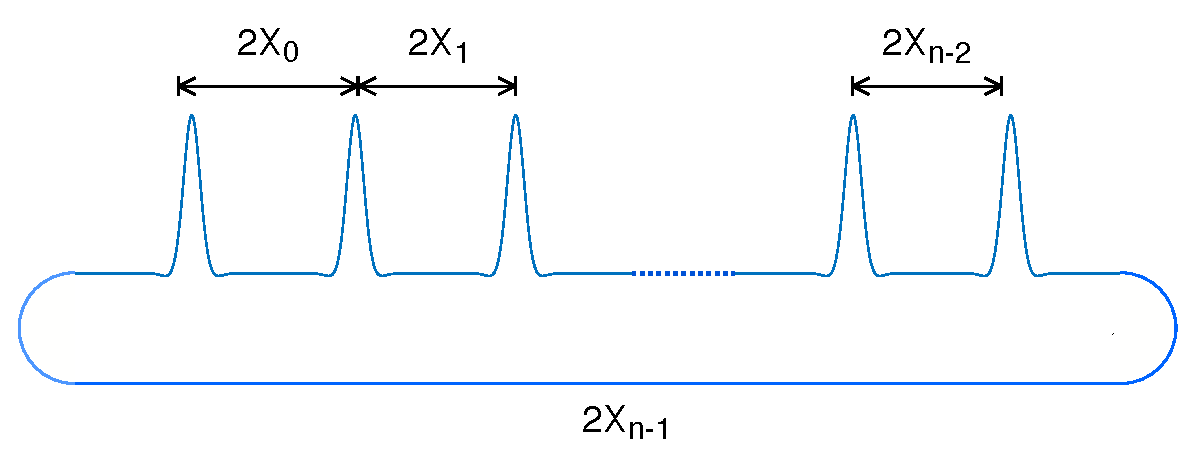
\includegraphics[width=10cm]{images/multipulseperiodic}
\end{center}
\caption[Construction of a periodic $n-$pulse solution]{Construction of a periodic $n-$pulse solution from the primary pulse.}
\label{fig:permultipulse}
\end{figure}
A periodic $n$-pulse can be described by $n$ pulse distances $\{X_0, \dots, X_{n-1} \}$, as shown in \cref{fig:permultipulse}, where the distance between consecutive copies of $Q(x)$ in the loop is $2 X_j$. The period of the orbit is $2X$, where $X = X_0 + \dots + X_{n-1}$. A periodic $n$-pulse requires one more pulse distance than an $n$-homoclinic orbit, since we need one more connection to ``close the loop''.  

Rather than describing a periodic multi-pulse by its physical pulse distances $X_j$, we will adopt an alternative parameterization which is both more convenient and captures the underlying geometry necessary for a periodic $n$-pulse to exist. This parameterization is an adaptation of that in \cite{SandstedeStrut,Sandstede1998} to the periodic case. Let
\begin{equation}\label{defrho}
\rho = \frac{\beta_0}{\alpha_0},
\end{equation}
where $\alpha_0$ and $\beta_0$ are defined in \cref{hypeqhyp}, and let
\begin{equation}\label{pstar}
p^* = \arctan \rho.
\end{equation}
Define the set
\begin{align}
\mathcal{R} &= \left\{ \exp\left(-\frac{2 k \pi}{\rho}\right) : k \in \N_0 \right\} \cup \{ 0 \},
\end{align}
which is a complete metric space. We will use $r \in \mathcal{R}$ as a scaling parameter. The parameterization is defined as follows.

\begin{definition}\label{def:perparam}
For $n \geq 2$, a \emph{periodic parameterization} of a periodic $n$-pulse is a sequence of parameters $(m_0, \dots, m_{n-1}, \theta)$, where
\begin{enumerate}[(i)]
\item $m_j$ is a nonnegative integer with
\begin{enumerate}
\item at least one of the $m_j \in \{0, 1\}$.
\item $m_{n-1} \geq m_j$ for $j = 0, \dots, n-2$.
\end{enumerate}
\item $\theta \in (\pi + -p^*, p^*]$.
\end{enumerate}
\end{definition}
The selection of $m_{n-1}$ as the largest of the $m_j$ is made only for notational convenience and to allow the parameterization to be unique. Since we are on a periodic domain, there is no loss of generality. The physical pulse distances $X_j$ are determined by these parameters and by the scaling parameter $r$. If $r = \exp\left(-\frac{2 k \pi}{\rho}\right)$, then
\begin{align*}
X_j &= \frac{1}{2 \beta_0}\big( (2 k + m_j)\pi + \theta^*(\theta; m_{n-1} - m_j)\big) + L_0 + \mathcal{O}(r) \\
X_{n-1} &= \frac{1}{2 \beta_0}\big( (2 k + m_{n-1})\pi + \theta \big) + L_0
\end{align*}
where $L_0$ is a constant. The functions $\theta^*(\theta; m): [-\pi + p^*, p^*] \rightarrow \R$ are defined for all nonnegative integers $m$, are continuous in $\theta$, and have the following properties.
\begin{enumerate}[(i)]
\item $\theta^*(0; m) = 0 \text{ for all } m$
\item $|\theta^*(\theta; m)| \leq |\theta|$
\item $|\theta^*(\theta; m)| \leq C \exp\left(-\frac{m \pi}{\rho} \right)$
\item $\theta^*(\theta; 0) = \theta $
\item $\theta^*(p^*; m) = \theta^*(-\pi+p^*; m+1)$ for $m \geq 1$
\end{enumerate}
The last property is a matching condition which ``links up'' the parameterizations corresponding to different $m_j$. These properties, together with the restriction of $\theta$ to the half-open interval $\theta \in (\pi + -p^*, p^*]$, guarantee that each periodic parameterization corresponds to a unique periodic multi-pulse. The proof that the functions $\theta^*(\theta; m)$ exist and have these properties is given in Lemma \ref{thetaparamlemma} below.

We can now state the main theorem of this section, which gives conditions for the existence of periodic multi-pulses. The requirement that the scaling parameter $r$ be sufficiently small means that the individual pulses must be well-separated.

\begin{theorem}[Existence of $n$-periodic solutions]\label{perexist}
Assume Hypotheses \ref{Ehyp}, \ref{Hhyp}, \ref{hypeqhyp}, \ref{Qexistshyp}, and \ref{H0transversehyp}. Let $Q(x)$ be the transversely constructed, symmetric primary pulse solution to \eqref{genODE} from Hypothesis \ref{Qexistshyp}. For any periodic parameterization $(m_0, \dots, m_{n-1}, \theta)$ with $\theta \notin \{-\pi + p^*, p^* \}$, there exists $r_* = r^*(m_0, \dots, m_{n-1}, \theta) > 0$ such that for any $r \in \mathcal{R}$ with $r \leq r_*$:
\begin{enumerate}[(i)]
	\item There exists a periodic $n$-pulse solution $Q_n(x) = Q_n(x; m_0, \dots, m_{n-1}, \theta, r)$ to \eqref{genODE}.

	\item The distances between consecutive copies of $Q(x)$ are $2X_j$, where
	\begin{align}\label{Xj}
		X_j(r; m_j, m_{n-1},\theta) &= \frac{1}{2 \alpha_0} |\log r| + \frac{1}{2\beta_0} t_j(r; m_j,m_{n-1}, \theta) + L_0 && j = 0, \dots, n-2 \\
		X_{n-1}(r; m_{n-1}, \theta) &= \frac{1}{2 \alpha_0} |\log r| + \frac{1}{2 \beta_0}\big( m_{n-1}\pi + \theta \big) + L_0.
	\end{align}
	The $t_j(r; m_j, m_{n-1}, \theta): \mathcal{R} \rightarrow \R$ are continuous in $r$ with 
	\[
	t_j(0; m_j, \theta) = m_j \pi + \theta^*(\theta; m_{n-1} - m_j),
	\]
	and $L_0$ is a constant.

	\item The periodic domain has length $2X$, where
	\begin{align}\label{Xdomain}
	X(r; m_0, \dots, m_{n-1}, \theta) = \frac{n}{2\alpha_0} |\log r| + \frac{1}{2\beta_0} \sum_{j=0}^{n-1} t_j(r; m_j, \theta) + n L_0
	\end{align}

	\item $Q_n(x)$ can be written as piecewise perturbation of the primary pulse $Q(x)$. 
	Details are given below in Lemma \ref{solvewithjumps}.
\end{enumerate}
\end{theorem}

The condition that $\theta \notin \{-\pi + p^*, p^*) \}$ in \cref{perexist} is used to avoid any bifurcation points which may arise in the construction. For periodic 2-pulses, we can use a symmetry argument to give a complete bifurcation picture. In the next theorem, we show that for periodic 2-pulses, asymmetric solutions ($X_0 \neq X_1$) bifurcate from symmetric solutions ($X_0 = X_1$) in a series of pitchfork bifurcations (\cref{fig:2pitch}, left panel). We note that \cref{2pulsebifurcation} uses a different parameterization than \cref{perexist} (\cref{fig:2pitch}, right panel).

\begin{figure}
\begin{center}
\begin{tabular}{cc}
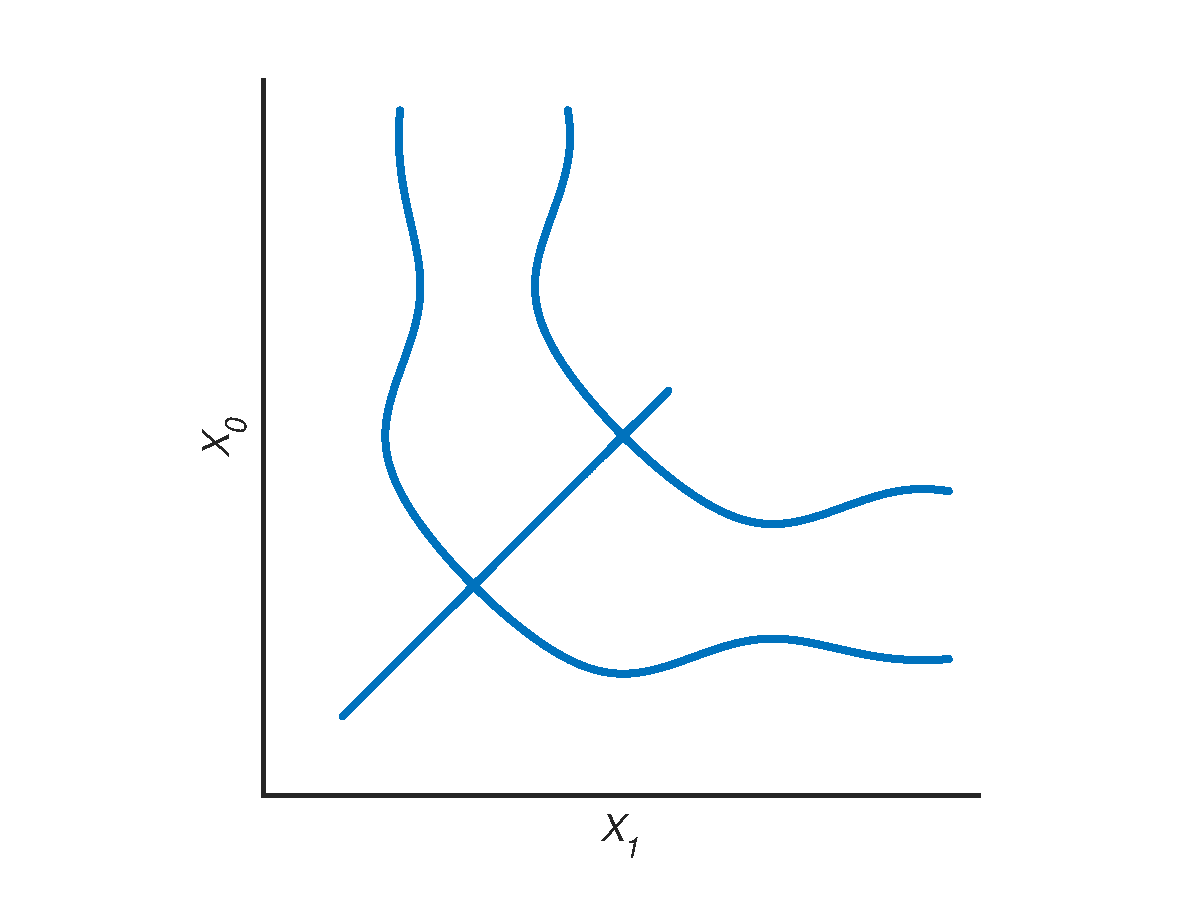
\includegraphics[width=8cm]{images/2pitchfork.eps}
\includegraphics[width=8cm]{images/2pitchparam1}
\end{tabular}
\end{center}
\caption[Pitchfork bifurcation structure for periodic 2-pulses]{Pitchfork bifurcation structure for periodic 2-pulses (right panel). Parameterization from \cref{2pulsebifurcation} (left panel). Symmetric periodic 2-pulses are in blue, and asymmetric periodic 2-pulses are in orange. Parameters $s_0$ and $s_1$ increase in the direction of the arrow.}
\label{fig:2pitch}
\end{figure} 

\begin{theorem}\label{2pulsebifurcation}
Assume Hypotheses \ref{Ehyp}, \ref{Hhyp}, \ref{hypeqhyp}, \ref{Qexistshyp}, and \ref{H0transversehyp}. Let $Q(x)$ be a transversely constructed, symmetric primary pulse solution to \eqref{genODE}. There exists $r_* > 0$ such that for all $r \in \mathcal{R}$ with $r \leq r_*$ and $m_0 \in \{0, 1\}$
\begin{enumerate}[(i)]
	\item There exists a family of symmetric periodic 2-pulses $\tilde{Q}_2(x; m_0, s_0, r)$ parameterized by $s_0 \in [0, \pi)$. The distances $\tilde{X}_j$ are given by
	\begin{equation}\label{2psymmdist}
		\tilde{X}_0(r, s_0) = \tilde{X}_1(r, s_0) = \frac{1}{2 \alpha_0} |\log r| + \frac{\pi}{2\beta_0} (m_0 + s_0) + L_0.
	\end{equation}
	\item There exists a family of asymmetric periodic 2-pulses $Q_2(x; m_0, s_1, r)$ with distances $X_1 > X_0$ parameterized by $s_1 \in [p^*, \infty)$. The distances $X_j$ are given by
	\begin{equation}\label{2pasymmdist}
	\begin{aligned}
		X_0(r, m_0, s_1) &= \frac{1}{2 \alpha_0} |\log r| + \frac{1}{2\beta_0} t_0(r; m_0, s_1) + L_0 \\
		X_1(r, s_1) &= \frac{1}{2 \alpha_0} |\log r| + \frac{1}{2\beta_0} s_1 + L_0, 
	\end{aligned}
	\end{equation}
	where $t_0(r; m_0, s_1)$ is continuous in $r$ and $t_1$, and $t_0(0; m_0, k \pi) = m_0$ for all nonnegative integers $k$. Furthermore,
	\begin{align}\label{deft0}
	t_0(0; m_0, s_1) = m_0 \pi + \mathcal{O}\left(-\frac{1}{\rho} s_1 \right)
	\end{align}
	The periodic domain has length $2X$, where
	\begin{equation}\label{X2pdomain}
	X(r, m_0, s_1) = \frac{1}{2 \alpha_0} 2 |\log r| + \frac{1}{2\beta_0} \left( t_0(r; m_0, s_1) + s_1\right) + 2 L_0.
	\end{equation}

	\item The two families meet at a pitchfork bifurcation. In terms of the two parameterizations, this occurs when $s_0 = p^*(m_0; r)$ and $s_1 = p^*$. The bifurcation points $p^*(m_0; r)$ are continuous in $r$, and
	\[
	p^*(m_0; r) \rightarrow \arctan \rho \text{ as }r \rightarrow 0.
	\]
\end{enumerate}
\end{theorem}

As a consequence of our analysis, we also note that periodic single pulse solutions exist for sufficiently small $r$.

\section{Spectrum of periodic multipulses}\label{sec:perstab}

We now look at the spectral stability of the periodic multi-pulses which we constructed in the previous section. Let $Q(x)$ be the primary pulse solution, and let $Q_n(x)$ be any periodic $n$-pulse solution constructed according to Theorem \ref{perexist} on periodic domain $[-X, X]$. It is natural to pose the PDE eigenvalue problem \cref{genPDEeigper} on the space of periodic functions $H^{2m}_{\text{per}}[-X,X]$, where
\[
H^{2m}_{\text{per}}[-X,X] = \left\{ f \in H^{2m}(\R) : f^{(k)}(-X) = f^{(k)}(X) \text{ for } k = 0, \dots, 2m \right\} 
\]
The norm on this space is the $H^{2m}$ norm restricted to $[-X, X]$. Using the notation in \cref{genPDEeig}, let
\begin{equation}\label{AQnlambda}
A(Q_n(x); \lambda) = A(Q_n(x)) + \lambda B.
\end{equation}
Then the PDE eigenvalue problem on $[-X, X]$ is equivalent to the first order system with periodic boundary conditions
\begin{equation}\label{PDEeigsystemper3}
\begin{aligned}
V'(x) &= A(Q_n(x); \lambda)V(x) \\
V(-X) &= V(X),
\end{aligned}
\end{equation}
where $V(x) \in C^0(\R,\R^{2m+1})$. Let $A(\lambda) = A(0; \lambda)$. By Lemma \ref{eigA0lemma}, $A(0)$ has a simple eigenvalue at 0. The next lemma states that for small $\lambda$, $A(\lambda)$ has a simple eigenvalue $\nu(\lambda)$ near 0. The proof is part of Lemma \ref{nulambdalemma} below.

\begin{lemma}\label{nulambdalemmasimple}
There exists $\delta_0 > 0$ such that for $|\lambda| < \delta_0$, the matrix $A(\lambda)$ has a simple eigenvalue $\nu(\lambda)$ near 0.
\end{lemma}

We will need one final hypothesis concerning a higher order Melnikov-type integral that appears in the stability theorem. In applications such as KdV5, numerical analysis suggests that \cref{Melnikov2hyp} is satisfied with $M > 0$.

\begin{hypothesis}\label{Melnikov2hyp}
The following higher order Melnikov integral is nonzero.
\begin{equation}\label{M2}
M = \int_{-\infty}^\infty \langle \Psi(x), B Q_c(x) \rangle dx =
\int_{-\infty}^\infty q(x) \partial_c q(x) dx \neq 0
\end{equation}
\end{hypothesis}

We can now state the main theorem of this section, which provides a condition for \cref{PDEeigsystemper3} to have a solution. Since the spatial dynamics formulation \cref{PDEeigsystemper3} is equivalent to the PDE eigenvalue problem, this allow us to find the eigenvalues of \cref{genPDEeigper}. This theorem is analogous to \cite[Theorem 2]{Sandstede1998}, except the matrix $S(\lambda)$ is replaced by a block matrix.

% block matrix theorem
\begin{theorem}\label{blockmatrixtheorem}
Assume Hypotheses \ref{Ehyp}, \ref{Hhyp}, \ref{hypeqhyp}, \ref{Qexistshyp}, and \ref{H0transversehyp}, \ref{Qclocalhyp}, and \ref{Melnikov2hyp}. Let $Q(x)$ be the primary pulse solution, and let $\Psi(x)$ be the solution to the adjoint variational equation from Lemma \ref{varadjsolutions}. Choose any periodic parameterization $(m_0, \dots, m_{n-1}, \theta)$ with $\theta \notin \{-\pi + p^*, p^* \}$, and let $r_*$ be as in \cref{perexist}. 

Choose any positive integer $N$. Then for any $r \leq r_*$ there exists $\delta(r,N)$, where $0 < \delta(r,N) < N/|\log r|$, with the following property. There exists a bounded, nonzero solution $V(x)$ of \cref{PDEeigsystemper3} for $|\lambda| < \delta(r,N)$ if and only if
\begin{equation}\label{blockmatrixcond}
E(\lambda) = \det S(\lambda) = 0.
\end{equation}
$S(\lambda)$ is the $(2n \times 2n)$ block matrix
\begin{equation}\label{blockeq}
S(\lambda) = 
\begin{pmatrix}
K(\lambda) -\frac{1}{2} \tilde{M} K_1(\lambda) + C_1 & -\lambda A_1 - \lambda^2 \tilde{M}^c I + D_1 \\
-\frac{1}{2} \lambda M^c K_1(\lambda) + C_2 & A - \lambda^2 MI + D_2
\end{pmatrix}
\end{equation}
The individual terms in $S(\lambda)$ are as follows.

\begin{enumerate}
\item $K(\lambda)$ is the periodic, bi-diagonal matrix
\begin{align*}
K(\lambda) =  
\begin{pmatrix}
e^{-\nu(\lambda)X_1} & & & & & -e^{\nu(\lambda)X_0} \\
-e^{\nu(\lambda)X_1} & e^{-\nu(\lambda)X_2} \\
& -e^{\nu(\lambda)X_2} & e^{-\nu(\lambda)X_3} \\
  & & \ddots & && \\
& & & & -e^{\nu(\lambda)X_{n-1}} & e^{-\nu(\lambda)X_0}
\end{pmatrix}.
\end{align*}
where $\nu(\lambda)$ is defined in Lemma \ref{nulambdalemmasimple}.

\item $K_1(\lambda)$ is the same matrix as $K(\lambda)$ with all terms positive, i.e. 
\begin{align*}
K_1(\lambda) =  
\begin{pmatrix}
e^{-\nu(\lambda)X_1} & & & & & e^{\nu(\lambda)X_0} \\
e^{\nu(\lambda)X_1} & e^{-\nu(\lambda)X_2} \\
& e^{\nu(\lambda)X_2} & e^{-\nu(\lambda)X_3} \\
 & & \ddots & &&   \\
& & & & e^{\nu(\lambda)X_{n-1}} & e^{\nu(\lambda)X_0}
\end{pmatrix}.
\end{align*}

\item $A$ is the symmetric banded matrix
\begin{align}\label{Asymm}
A &= \begin{pmatrix}
-a_{n-1} - a_0 & a_0 & & &  & a_{n-1}\\
a_0 & -a_0 - a_1 &  a_1 \\
& a_1 & -a_1 - a_2 &  a_2 \\
& \ddots & \ddots & \ddots \\
a_{n-1} & & & & a_{n-2} & -a_{n-2} - a_{n-1} \\
\end{pmatrix},
\end{align}
where
\begin{align*}
a_i &= \langle \Psi(X_i), Q'(-X_i) \rangle
\end{align*}

\item $A_1$ is the matrix
\begin{align*}
A_1 &= \begin{pmatrix}
q(X_0) - q(X_1) & q(X_1) &&& -q(X_0) \\
-q(X_1) & q(X_1) - q(X_2) & q(X_2) \\
& -q(X_2) & q(X_2) - q(X_3) & q(X_3) \\ && \ddots \\
\\
q(X_0) &&& -q(X_{n-1}) & q(X_{n-1}) - q(X_0) 
\end{pmatrix},
\end{align*}
where $q(x)$ is the first component of the primary pulse solution $Q(x)$. 

\item $M$, $M^c$, $\tilde{M}$, and $\tilde{M}^c$ are  Melnikov-type integrals
\begin{align*}
M &= \int_{-\infty}^\infty q(y) \partial_c q(y) dy \\
M^c &= \int_{-\infty}^\infty q(y) v^c(y) dy \\
\tilde{M} &= \int_{-\infty}^{\infty} \left(v^c(y) - \frac{1}{c}\right) dy \\
\tilde{M}^c &= \int_{-\infty}^\infty \partial_c q(y) dy
\end{align*}
where $v^c(y)$ is the first component of $V^c(y)$, which is defined in \cref{varadjsolutions}.

\item The remainder matrices and $K_2(\lambda)$ are analytic in $\lambda$ and have uniform bounds
\begin{align*}
|C_1| &\leq C |\lambda|(|\lambda| + r^{1/2}) \\
|D_1| &\leq C |\lambda|(|\lambda| + r^{1/2})^2 \\
|C_2| &\leq C (|\lambda| + r^{1/2})^2 \\
|D_2| &\leq C (|\lambda| + r^{1/2})^3 
\end{align*}
The constants $C$ depend on $N$.
\end{enumerate}
\end{theorem}

To leading order, equation \cref{blockeq} is block diagonal with blocks $A - \lambda^2 MI$ and $K(\lambda) -\frac{1}{2} \tilde{M} K_1(\lambda)$. Singularities of $A - \lambda^2 MI$ correspond to the interaction eigenvalues as well as two kernel eigenvalues. Singularities of $K(\lambda) -\frac{1}{2} \tilde{M} K_1(\lambda)$ correspond to the essential spectrum eigenvalues, as well as one additional kernel eigenvalue.

\begin{remark}
In \cref{blockmatrixtheorem}, we restricted $|\lambda|$ to $|\lambda| < N/|\log r|$, for a positive integer $N$ we choose. Without this restriction, the analysis is still possible, but the remainder terms in \cref{blockeq} are much more complicated. Since the essential spectrum eigenvalues are located at approximately $c\frac{k \pi i}{X}$ for $k \in \Z$, and \begin{align*}
\left| c\frac{k \pi i}{X} \right| \leq \frac{N}{|\log r|} && |k|\leq N,
\end{align*} 
the restriction $\delta(r,N) < N/|\log r|$ in \cref{blockmatrixtheorem} will not hinder a search for the first $N$ essential spectrum eigenvalues.
\end{remark}

\section{Spectrum of periodic pulses}

\subsection{Spectrum of periodic single pulse}\label{sec:per1peig}

The simplest case is the periodic single pulse. There is a only single length parameter $X_0$, which is the same as the domain length $X$. The block matrix $S(\lambda)$ is a $2\times 2$ matrix, the form of which is given in the next corollary.

\begin{corollary}\label{corr:2blockmatrix}
For a periodic single pulse, the block matrix $S(\lambda)$ from \cref{blockmatrixtheorem} is 
\begin{align}\label{1pblockmatrix}
S(\lambda) &= 
\begin{pmatrix}
-2 \sinh(\nu(\lambda) X) - \tilde{M}\lambda \cosh(\nu(\lambda) X) & -\tilde{M}^c \lambda^2 \\
-M^c \lambda \cosh(\nu(\lambda)X) & - M \lambda^2
\end{pmatrix} +
\begin{pmatrix}
C_1 & D_1 \\ C_2 & D_2
\end{pmatrix},
\end{align}
where
\begin{align*}
|C_1|, |C_2| &\leq C |\lambda|(|\lambda| + r^{1/2}) \\
|D_1|, |D_2| &\leq C |\lambda|^2(|\lambda| + r^{1/2})
\end{align*}
In addition,
\begin{equation}\label{1pblockmatrixdet}
\det S(\lambda, r) = \lambda^2 \left( 2 M \sinh(\nu(\lambda)X)(1 + \mathcal{O}(|\lambda| + r^{1/2})) + \lambda(M \tilde{M} - M_c \tilde{M}_c)\cosh(\nu(\lambda)X) + \mathcal{O}(|\lambda|(|\lambda| + r^{1/2}) \right)
\end{equation}
\begin{proof}
We use the same piecewise ansatz as in \cref{Vpiecewise}, and we note that that there is only one parameter $c$ and one parameter $d$. The system of equations \cref{eigsystem} becomes
\begin{equation}\label{eigsystemper1p}
\begin{aligned}
(W^\pm)'(x) &= A(Q(x); \lambda) W^\pm(x) + G^\pm(x) W^\pm(x) + c e^{\mp\nu(\lambda)X} G^\pm(x)V^\pm(x; \lambda) + d \lambda^2 \tilde{H}^\pm(x) \\
W^+(X) &- W^-(-X) = C_i c \\
W^\pm(0) &\in \R \Psi(0) \oplus \R \Psi^c(0) \oplus Y^+ \oplus Y^- \\
W^+(0) &- W_i^-(0) \in \R \Psi(0) \oplus \R \Psi^c(0) 
\end{aligned}
\end{equation}
In particular, the second equation in \cref{eigsystemper1p} (the matching condition at the tail) no longer contains the term $D_i d$. Since the periodic single pulse is symmetric, $Q^-(x) = R Q^+(-x)$. Following the same procedure as in \cref{AQxsymmetrylemma}, it follows that $G^-(x) = -R G^+(-x)R$. Multiplying the first equation in \cref{eigsystemper1p} by $R$ on the right and using the symmetry relations,
\begin{align*}
(R W^\pm)'(x) &= R A(Q(x); \lambda) R R W^\pm(x) + R G^\pm(x) R R W^\pm(x) + c e^{\mp\nu(\lambda)X} R G^\pm(x)R R V^\pm(x; \lambda) + d \lambda^2 R \tilde{H}^\pm(x) \\
&= -A(Q(-x); -\lambda) R W^\pm(x) - G^\mp(-x) R W^\pm(x) - c e^{\pm\nu(-\lambda)X} G^\mp(-x) V^\mp(-x; -\lambda) + d \lambda^2 \tilde{H}^\mp(-x)
\end{align*}
Making the change of variables $x \mapsto -x$, this becomes
\begin{align*}
[-R W^\mp(-x)]' &= A(Q(x); -\lambda)[ R W^\mp(-x)] + G^\pm(x) [-R W^\mp(-x)] - c e^{\mp\nu(-\lambda)X} G^\pm(x) R V^\pm(x; -\lambda) + d \lambda^2 \tilde{H}^\pm(x)
\end{align*}
Multiplying the second equation in \cref{eigsystemper1p} by $R$,
\begin{align*}
RW^+(X) - RW^-(-X) &= c \left( e^{\nu(\lambda) X_i} R V^-(-X_i; \lambda) - e^{-\nu(\lambda) X_i} R V^+(X_i; \lambda) \right) \\
 [-RW^-(-X)] - [-RW^+(X)]&= -c \left( e^{\nu(-\lambda) X_i} V^-(-X_i; -\lambda) - e^{-\nu(-\lambda) X_i} V^+(X_i; -\lambda) \right)
\end{align*}
Since $Y^+ = R Y^-$, $R \Psi(0) = \Psi(0)$, and $R \Psi^c(0) = \Psi^c(0)$, the system of equations \cref{eigsystemper1p} is satisfied by $(-RW^-(-x), -RW^+(-x))$ when $(c, d, \lambda) \mapsto (-c, d, -\lambda)$. Since the solution $(W^+(x), W^-(x))$ is unique for a given $(c, d, \lambda)$, 
\[
\left(W^+(x; c, d, -\lambda), W^-(x; -c, d, -\lambda)\right)
= -\left(RW^-(-x; c, d, \lambda), RW^+(-x; -c, d, \lambda)\right)
\]




Equation \cref{1pblockmatrix} then follows directly from \cref{blockmatrixtheorem}. For the remainder bounds, we first note that since $D_i d = 0$, the parameter $d$ only 

\end{proof}
\end{corollary}

\begin{theorem}\label{theorem:1pess}
Assume Hypotheses \ref{Ehyp}, \ref{Hhyp}, \ref{hypeqhyp}, \ref{Qexistshyp}, \ref{H0transversehyp}, \ref{Melnikov2hyp}, and \ref{Hoverlaphyp}. Let $r_*$ be as in \cref{2pulsebifurcation}. Choose any integer $N > 0$, and let $\delta(N,r)$ be as in Theorem \ref{blockmatrixtheorem}. Then there exists $r_1 \leq r_*$ such that for any $r \in \mathcal{R}$ with $r \leq r_1$, the following holds regarding the nonzero essential spectrum eigenvalues. 

Let $N_1 \leq N$ be the largest positive integer such that $N_1/|\log r| < \delta(N,r)$. Then there are $2N_1$ nonzero essential spectrum eigenvalues $\lambda = \{ \pm \lambda_m^{\text{ess}} : m = 1, \dots, N_1 \}$, where
\[
\lambda_m^{\text{ess}}(r) = c \frac{m \pi i}{X + c \frac{M\tilde{M} - M_c\tilde{M_c}}{2 M}} +  \mathcal{O}\left( \frac{1}{|\log r|^2} \right)
\]
is on the imaginary axis.
\begin{proof}
First, we make a change of variables to simplify the problem. Since $\nu'(0) = 1/c$ and $\nu(0) = 0$, $\nu(\lambda)$ is invertible near 0. Let $\lambda = \nu^{-1}(\mu)$. Expanding in Taylor series about $\mu = 0$,
\begin{equation}\label{2plambdamu}
\lambda = \nu^{-1}(\mu) = c \mu + \mathcal{O}(\mu^3)
\end{equation}
Substituting this into \cref{1pblockmatrixdet} and simplifying, we obtain the equation
\begin{equation}\label{1pdetmu}
\det S(\mu, r) = c^2 \mu^2 \left( 2 M \sinh(\mu X)(1 + \mathcal{O}(|\mu| + r^{1/2})) + c \mu (M \tilde{M} - M_c \tilde{M}_c)\cosh(\mu X) + \mathcal{O}(|\mu|(|\mu| + r^{1/2}) \right)
\end{equation}
For convenience, let $K = M \tilde{M} - M_c \tilde{M}_c$. Since we are looking for the nonzero essential spectrum eigenvalues, and we know there is an eigenvalue with algebraic multiplicity 2 at 0, we divide by $c \mu^2$ to get the equation
\begin{equation}\label{1pdetmu2}
E(\mu, r) = 2 M \sinh(\mu X)(1 + \mathcal{O}(|\mu| + r^{1/2})) + c K \mu \cosh(\mu X) + \mathcal{O}(|\mu|(|\mu| + r^{1/2})
\end{equation}
Choose positive integer $m \leq N_1$. Then for our ansatz, we let
\begin{equation}
\mu = \frac{m \pi i}{X + c \frac{K}{2 M}} + \frac{h}{X^2}
\end{equation}
Factoring out an $X$ in the denominator, and expanding the denominator in a Taylor series, which we can do for sufficiently large $X$,
\begin{align*}
\mu &= \frac{m \pi i}{X\left(1  + c \frac{K}{2 M X} \right) } + \frac{h}{X^2}\\
&= \frac{m \pi i}{X}\left( 1 - c \frac{K}{2 M X} + c^2 \frac{K^2}{4 M^2 X^2} + \mathcal{O}\left(\frac{1}{X^3}\right) \right) + \frac{h}{X^2}
\end{align*}
Substituting this into \cref{1pdetmu2} and expanding the $\sinh$ and $\cosh$ terms in a Taylor series about $m \pi i$,
\begin{align*}
E(\mu, r) = 2 M \sinh(\mu X)(1 + \mathcal{O}(|\mu| + r^{1/2})) + c K \mu \cosh(\mu X) + \mathcal{O}(|\mu|(|\mu| + r^{1/2})
\end{align*}
\end{proof}
\end{theorem}




\section{Spectrum of periodic 2-pulse}\label{sec:per2peig}

We will apply \cref{blockmatrixtheorem} to the simplest case, which is the periodic 2-pulse. The block matrix $S(\lambda)$ is a $4\times 4$ matrix, the form of which is given in the next corollary, which follows immediately from \cref{blockmatrixtheorem}.

\begin{corollary}\label{corr:2blockmatrix}
For a periodic 2-pulse, the block matrix \cref{blockeq} from \cref{blockmatrixtheorem} can be written as $S(\lambda) = S_1(\lambda) + S_2(\lambda)$. $S_1(\lambda)$ is the $4 \times 4$ matrix
\begin{align}
S&_1(\lambda) = \\
&\begin{pmatrix}
e^{-\nu(\lambda)X_1} & -e^{\nu(\lambda)X_0} & k_0^+ - k_1^- -\tilde{M}^c \lambda^2 & -k_0^+ + k_1^- \\
-e^{\nu(\lambda)X_1} & e^{-\nu(\lambda)X_0} & k_0^- - k_1^+ & -k_0^- + k_1^+-\tilde{M}^c \lambda^2 \\
-\frac{1}{2}\lambda M^c e^{-\nu(\lambda)X_1} & -\frac{1}{2}\lambda M^ce^{\nu(\lambda)X_0} &-a-\lambda^2 M_2 & a \\
-\frac{1}{2}\lambda M^c e^{\nu(\lambda)X_1} & -\frac{1}{2}\lambda M^c e^{-\nu(\lambda)X_0}  & a & -a-\lambda^2 M_2 \\
\end{pmatrix}
\end{align}
where
\begin{equation}\label{2pa}
a = \langle \Psi(X_0), Q'(-X_0) \rangle + \langle \Psi(X_1), Q'(-X_1) \rangle
\end{equation}
and the rest of the terms are defined in \cref{blockmatrixtheorem}. $S_2(\lambda)$ is the remainder matrix
\[
S_2(\lambda) = \begin{pmatrix} C_1 & D_1 \\ C_2 & D_2 \end{pmatrix}.
\]
The remainder terms have the same bounds as in \cref{blockmatrixtheorem}.
\end{corollary}

With the aid of Mathematica, the determinant of the block matrix for the periodic 2-pulse is a straightforward computation.

\begin{corollary}\label{corr:2perDet1}
For a periodic 2-pulse, the determinant of the block matrix $S(\lambda)$ is given by
\begin{equation*}
\begin{aligned}
\det S(&\lambda) = -2 \lambda^2 M (2a + \lambda^2 M) \sinh(\nu(\lambda)X) + R(\lambda),
\end{aligned}
\end{equation*}
where the remainder term have bounds
\begin{align*}
|R(\lambda)| \leq C(r^{1/2} + |\lambda|)^5
\end{align*}
\end{corollary}

The interaction eigenvalue pattern will be determined by the quantity $a$ in \cref{2pa}. In order to characterize this, we will need to make one technical hypothesis. Define the functions $H: \R^+ \times \R^+ \rightarrow \R$ and $K: \R^+ \times \R^+ \rightarrow \R$ by 
\begin{align}
H(b_0, b_1) &= b_0 \sin \left( -\rho \log b_0 \right) - b_1 \sin \left( -\rho \log b_1 \right) \label{perdefH} \\
H_1(b_0, b_1) &= b_0 \left[ \rho \cos \left( -\rho \log b_0 \right) - \sin \left( -\rho \log b_0 \right) \right] + b_1 \left[ \rho \cos \left( -\rho \log b_1 \right) - \sin \left( -\rho \log b_1 \right) \right]  \label{perdefH1} \\
\end{align}
Roughly speaking, the permissible pulse distances for periodic 2-pulses are determined by the zero set of $H(b_0, b_1)$. 
% See \cref{section:bifH} for details. 
The value of $a$ is determined by $H_1(b_0, b_1)$ evaluated on the zero set of $H(b_0, b_1)$. We hypothesize that the zero sets of these two functions overlap only at a discrete set of points corresponding the pitchfork bifurcation points in \cref{2pulsebifurcation}.

\begin{hypothesis}\label{Hoverlaphyp}
The zero sets of $H(b_0, b_1)$ and $H_1(b_0, b_1)$ intersect only at the discrete set of points
\begin{align*}
(b_0, b_1) &= (b_k^*, b_k^*) && k \in \Z
\end{align*}
where 
\begin{equation*}
b^*_k = e^{-\frac{1}{\rho} (k \pi + p^*) }
\end{equation*}
These are the same as the pitchfork bifurcation points from \cref{2pulsebifurcation}.
\end{hypothesis}

% \begin{remark}There is strong numerical evidence that \cref{Hoverlaphyp} is true. See \cref{fig:HH1overlap} for a plot of two zero sets. Although it is likely that \cref{Hoverlaphyp} can be proved, the functions involved, while smooth, are not well-behaved, making the analysis very difficult.
% \end{remark}

% \begin{figure}
% \begin{center}
% \begin{tabular}{cc}
% \includegraphics[width=10cm]{images/periodic/zeroHoverlap.eps} 
% \end{tabular}
% \end{center}
% \caption[Intersection of zero sets of $H$ and $H_1$]{ Intersection of zero sets of $H(b_0, b_1)$ (blue) and $H_1(b_0, b_1)$ (orange). }
% \label{fig:HH1overlap}
% \end{figure}

We can now characterize the quantity $a$ in \cref{2pa} from \cref{corr:2blockmatrix}.

\begin{lemma}\label{lemma:chara}
Let $r_*$ be as in Theorem \ref{2pulsebifurcation}. Then for any $r \in \mathcal{R}$ with $r \leq r_*$:
\begin{enumerate}[(i)]
	\item For a symmetric periodic 2-pulse $\tilde{Q}_2(x; m_0, s_0, r)$, $a = r \tilde{a}(r; m_0, s_0)$, where $\tilde{a}(r; m_0, s_0)$ is continuous in $r$. Furthermore $\tilde{a}(0; m_0, s_0) = 0$ if and only if $s_0 = p^*$. For $s_0 \neq p^*$,
	\begin{equation}
	\begin{aligned}
	\text{if }s_0 &> p^*, \, \tilde{a}(0; 0, s_0) > 0 \text{ and } \tilde{a}(0; 1, s_0) < 0 \\
	\text{if }s_0 &< p^*, \, \tilde{a}(0; 0, s_0) < 0 \text{ and } \tilde{a}(0; 1, s_0) > 0 
	\end{aligned}
	\end{equation}

	\item For an asymmetric periodic 2-pulse $Q_2(x; m_0, s_1, r)$, $a = r \tilde{a}(r; m_0, s_1)$, where $\tilde{a}(r; m_0, s_0)$ is continuous in $r$. The sign of $\tilde{a}(r; m_0, s_0)$ is completely determined by $m_0$ as follows.
	\begin{equation} 
	\begin{aligned}
	\tilde{a}(0; m_0, s_1) &< 0 && \text{if }m_0 = 0 \\
	\tilde{a}(0; m_0, s_1) &> 0 && \text{if }m_0 = 1
	\end{aligned}
	\end{equation}
	Furthermore,
	\begin{equation}\label{tildeas1limit}
	\tilde{a}(r; m_0, s_1) = \tilde{a}^*(m_0) + \mathcal{O}\left(r^{\gamma/2\alpha_0} + e^{-\frac{1}{\rho}s_1} \right),
	\end{equation}
	where $\gamma > 0$. Finally, $\tilde{a}^*(m_0) < 0$ if $m_0 = 0$ and $\tilde{a}^*(m_0) > 0$ if $m_0 = 1$.
\end{enumerate}	
\end{lemma}

We will consider only the case where the interaction eigenvalues are ``out of the way'' of the essential spectrum eigenvalues. Since the interaction eigenvalues scale like $r^{1/2}$ and the essential spectrum eigenvalues scale like $1/|\log r|$, we can always choose $r$ sufficiently small so that this is the case. 
%In particular, this will always avoid the Krein bubbles that we observed numerically in \cref{chapter:KdV5numerics}. We will discuss the Krein bubbles in the concluding chapter. We expect that the eigenvalues will come in one of the two patterns shown in \cref{fig:2ppatterns}.

% \begin{figure}
% \begin{center}
% \begin{tabular}{cc}
% \includegraphics[width=5cm]{images/kdv5/2punstableeigpattern.eps} &
% \includegraphics[width=5cm]{images/kdv5/2pstableeigpattern.eps} 
% \end{tabular}
% \caption[Eigenvalue patterns for periodic 2-pulses]{Eigenvalue patterns for periodic 2-pulses with essential spectrum out of the way. Blue dots are interaction eigenvalues, red dots are essential spectrum eigenvalues, and black X at the origin represents the three kernel eigenvalues. Left panel shows a pair of real interaction eigenvalues, and right panel shows a pair of purely imaginary interaction eigenvalues.}
% \label{fig:2ppatterns}
% \end{center}
% \end{figure}

We will state the result separately for asymmetric and symmetric periodic 2-pulses. First, we locate the eigenvalues for asymmetric 2-pulses. As long as $r$ is chosen sufficiently small, the interaction eigenvalue pattern is determined by the parameter $m_0$, and the essential spectrum eigenvalues do not interfere.

\begin{theorem}\label{theorem:2peigsassym}
Assume Hypotheses \ref{Ehyp}, \ref{Hhyp}, \ref{hypeqhyp}, \ref{Qexistshyp}, \ref{H0transversehyp}, \ref{Melnikov2hyp}, and \ref{Hoverlaphyp}. Let $r_*$ be as in \cref{2pulsebifurcation}. Let $\tilde{a}(r)$ be as in \cref{lemma:chara}. Choose any integer $N > 0$, and let $\delta(N,r)$ be as in Theorem \ref{blockmatrixtheorem}. Then for every $m_0 \in \{0, 1\}$ and $s_1 > p^*$ there exists $r_1 = r_1(m_0, s_1, N) \leq r_*$ with the following property. For any $r \in \mathcal{R}$ with $r \leq r_1$, the following hold regarding the spectrum associated with the asymmetric periodic 2-pulse $Q_2(x; m_0, s_1, r)$.

\begin{enumerate}[(i)]
\item There is an eigenvalue at 0 with algebraic multiplicity 3. 
\item Let $N_1 \leq N$ be the largest positive integer such that $N_1/|\log r| < \delta(N,r)$. Then there are $2N_1$ nonzero essential spectrum eigenvalues $\lambda = \{ \pm \lambda_m^{\text{ess}} : m = 1, \dots, N_1 \}$, where
\[
\lambda_m^{\text{ess}}(r) = c \frac{m \pi i}{X}+  \mathcal{O}\left( \frac{1}{|\log r|^2} \right)
\]
is on the imaginary axis and $X$ is given by \cref{Xdomain}.

\item There is a pair of interaction eigenvalues located at $\lambda = \pm \lambda^{\text{int}}(r)$, where
	\begin{align*}
	\lambda^{\text{int}}(r) =  \sqrt{-\frac{2 \tilde{a}(r)}{M}}r^{1/2} + \mathcal{O}\left( \frac{r^{1/2}}{|\log r|} \right) 
	\end{align*}
and $|\lambda^{\text{int}}(r)| < \frac{1}{2}|\lambda_1^{\text{ess}}(r)|$. If $M > 0$, these are real when $m_0 = 0$ and purely imaginary when $m_0 = 1$. (This is reversed if $M < 0)$. 
\item There are no other eigenvalues inside a circle with radius slightly larger than $|\lambda_{N_1}^{\text{ess}}(r)|$.
\end{enumerate}
\end{theorem}

Next, we consider the symmetric periodic 2-pulse. As long as we are away from the pitchfork bifurcation points, i.e. as long as $\tilde{a}(0) \neq 0$, the results of \cref{theorem:2peigsassym} hold in the symmetric case as well; the only difference is that the eigenvalue pattern is determined by the sign of $\tilde{a}_0(0)$ rather than by $m_0$. Thus we only need to consider what happens at the pitchfork bifurcation point.

\begin{theorem}\label{theorem:2peigssym}
Assume Hypotheses \ref{Ehyp}, \ref{Hhyp}, \ref{hypeqhyp}, \ref{Qexistshyp}, \ref{H0transversehyp}, \ref{Melnikov2hyp}, and \ref{Hoverlaphyp}. Let $r_*$ be as in \cref{2pulsebifurcation}. Then there exists $r_1 \leq r_*$ such that for all $r \in \mathcal{R}$ with $r \leq r_1$ and for $m_0 \in \{0, 1\}$, there is eigenvalue at 0 with algebraic multiplicity 5 for the symmetric periodic 2-pulse $\tilde{Q}_2(x; m_0, p^*(r), r)$.
\end{theorem}

\section{Spectrum of periodic multi-pulses}

When $n \geq 3$, it should be possible to prove an analogue to \cref{theorem:2peigsassym} in the case where the essential spectrum eigenvalues and nonzero interaction eigenvalues do not interfere with each other. Since it is too unwieldy to compute the determinant, we note that it follows from Theorem \ref{blockmatrixtheorem} that $\lambda$ is an eigenvalue if and only if the equation
\[
S(\lambda) \begin{pmatrix} c\\d \end{pmatrix} = 0
\]
has a nontrivial solution. Write this as the pair of equations
\begin{align}
(K(\lambda) + C_1)c + (\lambda K_2(\lambda) - \lambda^2 \tilde{M}^c I + D_1)d &= 0 \label{topline} \\
(-\frac{1}{2} \lambda M^c K_1(\lambda) + C_2)c + (A - \lambda^2 MI + D_2) &= 0 \label{bottomline}.
\end{align}
To find the interaction eigenvalues, it should be possible to invert $K(\lambda)$, solve \cref{topline} for $c$, and plug the result into \cref{bottomline}. To find the essential spectrum eigenvalues, it should be possible to invert $A - \lambda^2 MI$, solve \cref{bottomline} for $d$, and plug the result into \cref{topline}.

\section{Numerical Results}

In this section, we present numerical results for the existence and spectrum of periodic multi-pulse solutions to \cref{KdV5c}. We start with the construction of the primary pulse solution. For $c = 36/169 < 1/4$, an exact solution to \cref{KdV5eq4} is known \cite[(3)]{Pelinovsky2007}:
\begin{equation}\label{KdV5exactsol}
q(x) = \frac{105}{338}\sech^4\left(\frac{x}{2\sqrt{13}} \right)
\end{equation}
By \cite{Pelinovsky2007}, multi-pulses exist when $c > 1/4$, and we will show that periodic multi-pulses also exist for $c > 1/4$. To obtain a primary pulse solution for $c > 1/4$, we use AUTO for parameter continuation in $c$ starting with the solution \cref{KdV5exactsol} at $c = 36/169$. Since we will are interested in periodic solutions, we use periodic boundary conditions on the bounded interval $[-X,X]$. (To do this in AUTO, we scale equation \cref{KdV5eq4} from $[-X, X]$ to $[0, 1]$ by taking $x \mapsto \frac{1}{2X}(x + X)$). Following the AUTO demo \texttt{kdv}, we use the Hamiltonian formulation \cref{KdV5ham2} and include a small parameter $\epsilon$ to break the Hamiltonian structure. In \cref{fig:KdV5singlepulse}, we plot the exact solution (left) together with the output of parameter continuation for $c = 10$ (right). We note the presence of oscillatory tails for $c = 10$ (these are hard to see since the tails also decay exponentially, but the first downward bump is visible).
\begin{figure}
\begin{center}
\begin{tabular}{cc}
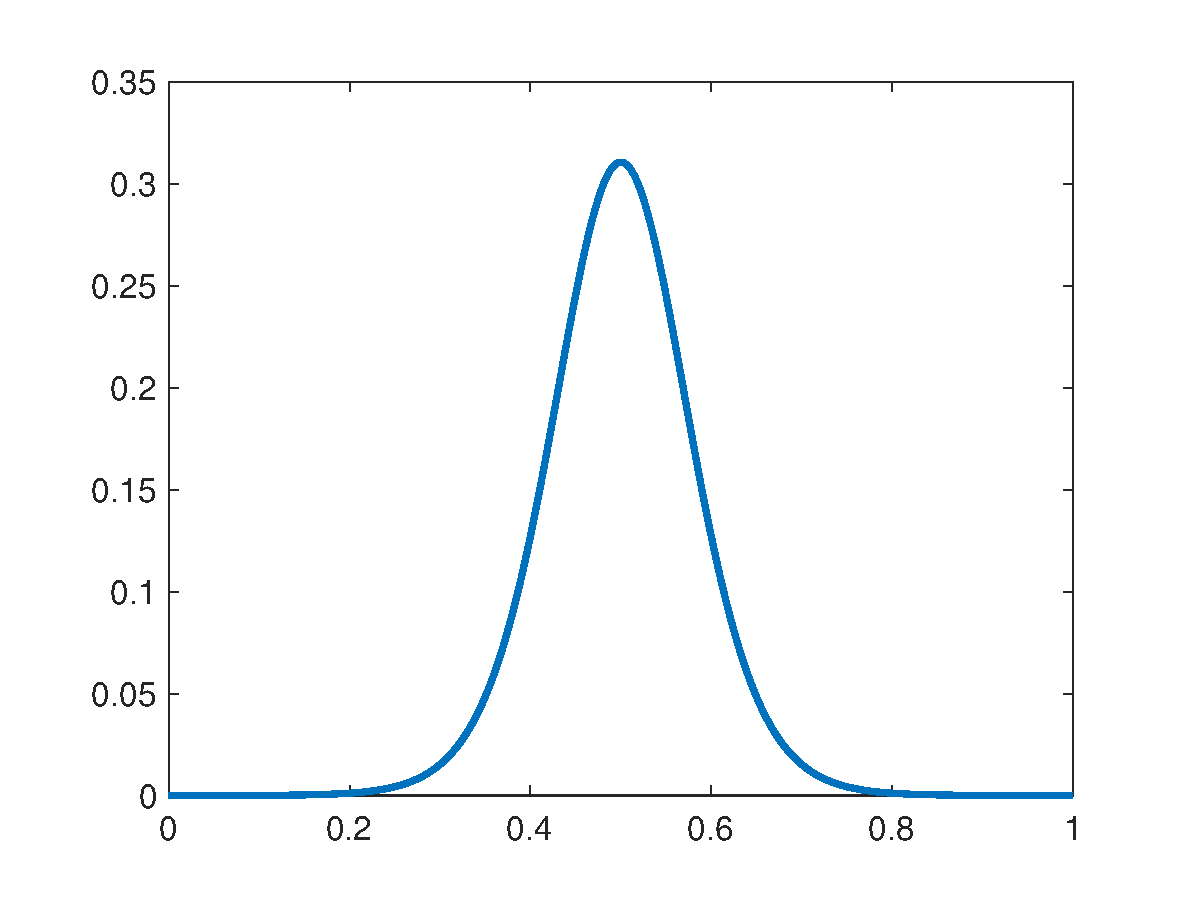
\includegraphics[width=7cm]{images/singleexact.eps} &
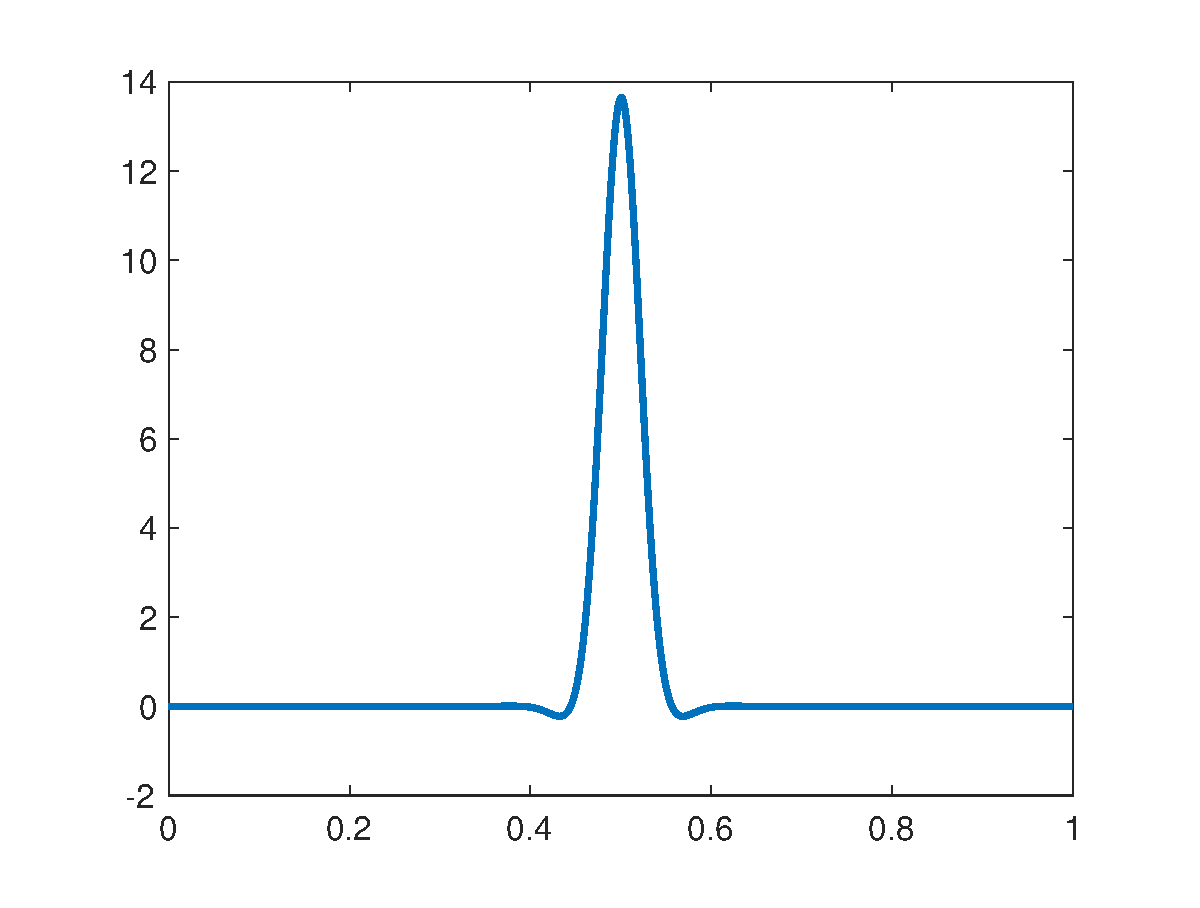
\includegraphics[width=7cm]{images/single10}
\end{tabular}
\caption[Primary pulse solutions for KdV5]{Single pulse solutions for KdV5. Exact solution for $c = 36/169$ (left panel) and solution from parameter continuation using AUTO for $c = 10.0$ (right panel). Solutions have been scaled to $[0, 1]$ using $X = 25$ in both cases, periodic boundary conditions.}
\label{fig:KdV5singlepulse}
\end{center}
\end{figure}

To construct a periodic double pulse, we glue together two copies of the single pulse we constructed above. To enforce periodic boundary conditions, we use Fourier spectral methods for spatial discretization. As an initial ansatz, we splice two single pulses together. For the distance between the two peaks, we use those predicted by \cite{SandstedeStrut}; we choose $X$ sufficiently large so that the tail interactions at periodic boundary conditions do not affect the solution very much. The periodic double pulse is then found using Matlab's \texttt{fsolve} function (Levenberg–Marquardt algorithm). The first six periodic double pulse solutions are shown in \cref{fig:KdV5doublepulse}.
\begin{figure}
\begin{center}
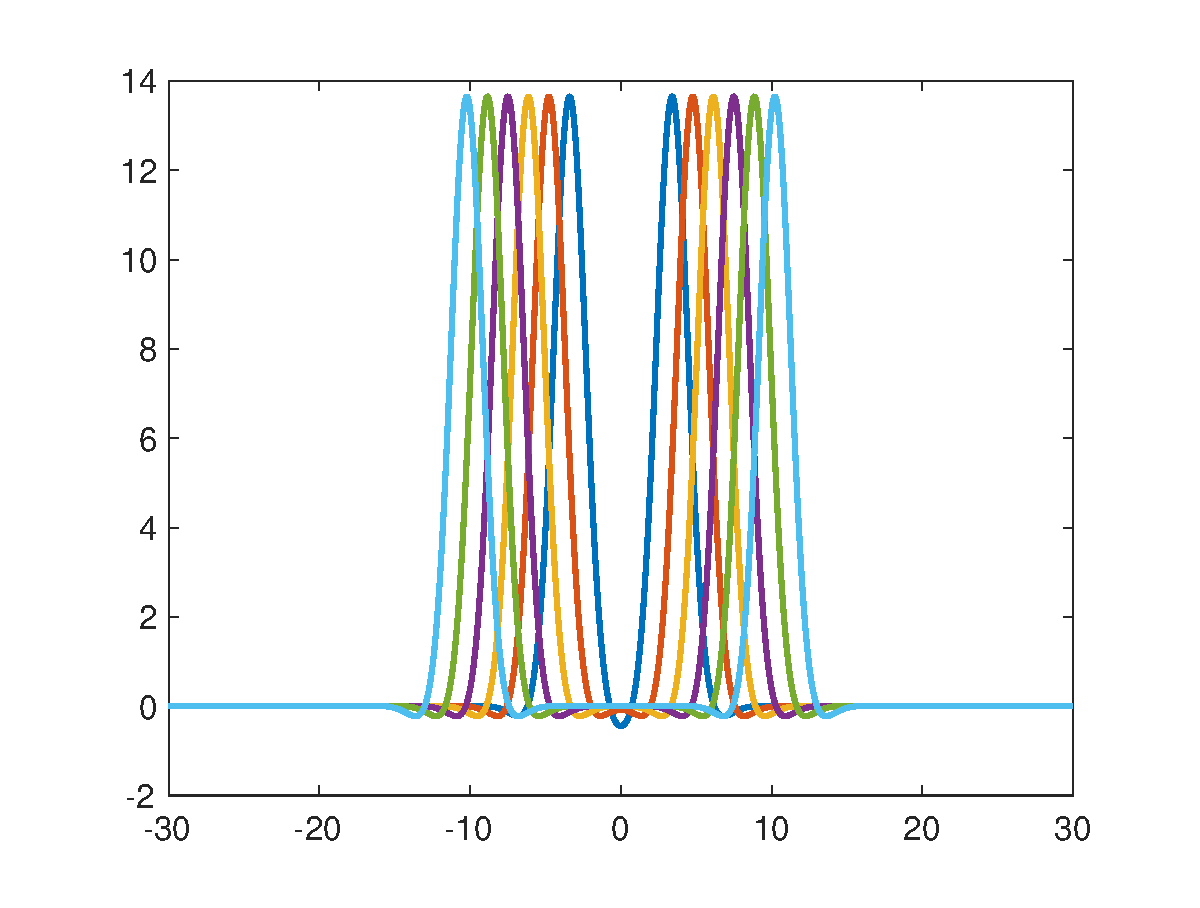
\includegraphics[width=7cm]{images/double10.eps}
\caption[Double pulse solutions for KdV5]{First six periodic double pulse solutions for KdV5. Fourier spectral methods with $N = 1024$ grid points, $c = 10$, $X = 25$.}
\label{fig:KdV5doublepulse}
\end{center}
\end{figure}
This same procedure can be used to construct arbitrary periodic multi-pulses. Once a periodic double pulse has been constructed, we can vary $X$ by using AUTO for parameter continuation. Transforming back from the interval $[0, 1]$ to $[-X, X]$, we plot the pulse distances $2 X_0$ vs $2 X_1$ in \cref{fig:periodicpitchfork}.
\begin{figure}
\begin{center}
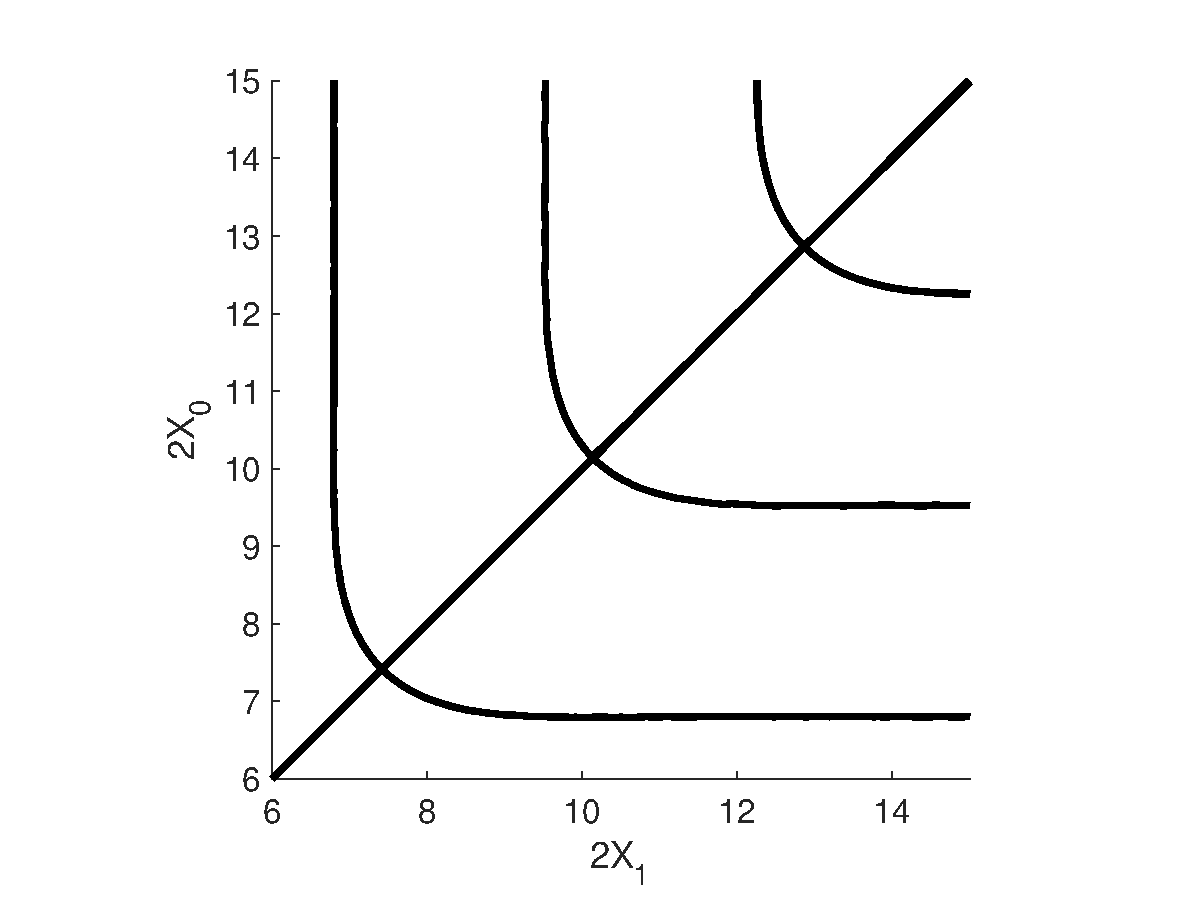
\includegraphics[width=10cm]{images/periodicpitchfork.eps}
\end{center}
\caption[Pulse distances of periodic multi-pulses in KdV5]{Pulse distances $2 X_0$ vs $2 X_1$ for periodic double pulse solutions to \cref{KdV5eq4}. Solutions with unequal pulse distances corresponding to the first three double pulses are shown in blue. Solutions with equal pulse distances are shown in red.}
\label{fig:periodicpitchfork}
\end{figure}
From this figure, we see that solutions with unequal pulse distances bifurcate from solutions with equal pulse distances in a series of pitchfork bifurcations. 

Now that we have constructed multi-pulses, we can look at their spectral stability. For a periodic double pulse $q_2$, we compute the spectrum of $\partial_x \calE''(q_n)$ numerically by writing the linear operator in matrix form using Fourier differentiation matrices and computing the eigenvalues of the resulting matrix using Matlab's \texttt{eig} function. On a periodic domain, the essential spectrum becomes a collection of discrete, purely imaginary eigenvalues. These eigenvalues depend only on the size of the periodic domain $X$ and are located at approximately
\begin{equation}\label{Kdv5peress}
\lambda \approx \left\{ c \frac{k \pi i}{L} : k \in \Z \right\} ,
\end{equation}
where $c$ is the wavespeed.

Next, we compute the interaction eigenvalues for periodic double pulses with equal pulse distances. We can identify the interaction eigenvalues because they correspond to localized eigenfunctions. For periodic double pulses with equal pulse distances ($X_1 = X_2$), the result is shown in \cref{fig:periodicequaleigbif}.
\begin{figure}
\begin{center}
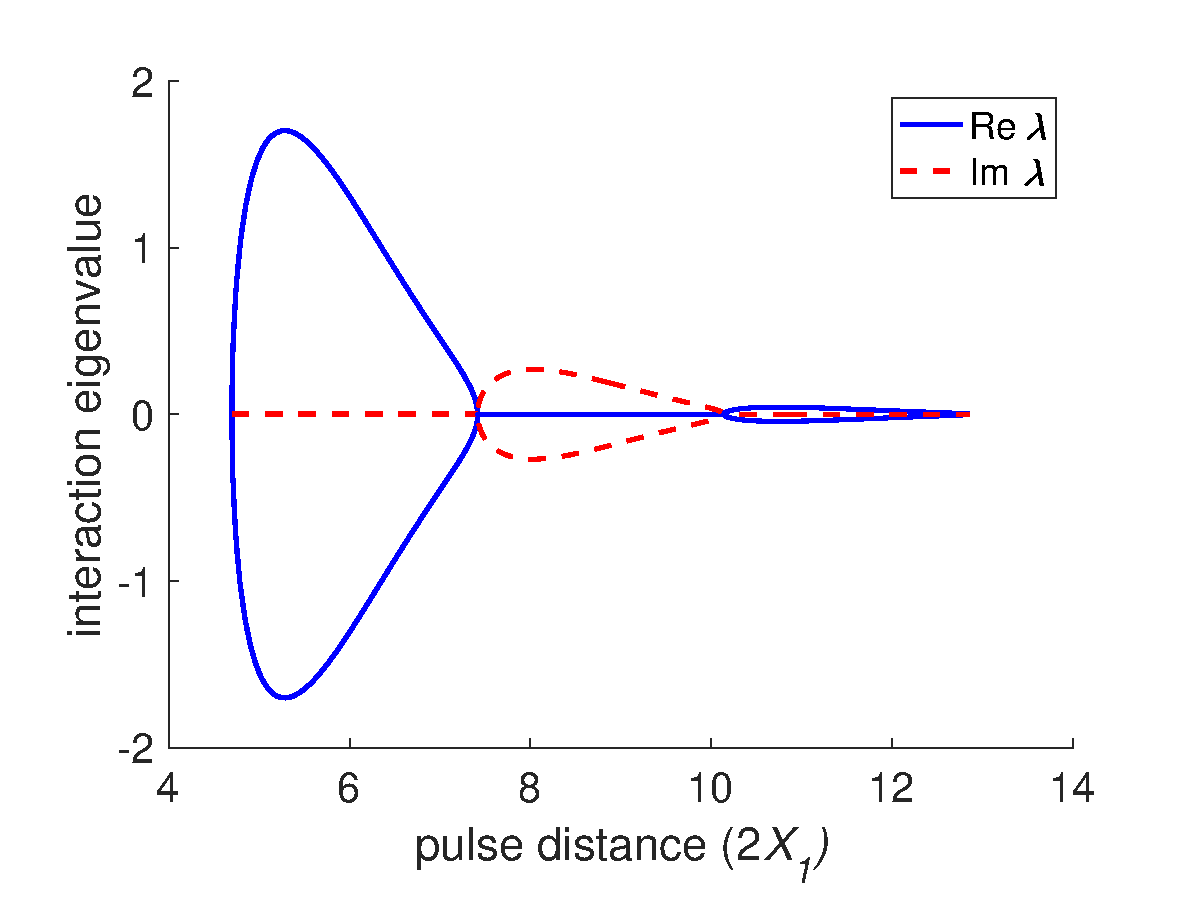
\includegraphics[width=10cm]{images/periodicequaleigbif.eps}
\end{center}
\caption[Eigenvalue bifurcations for symmetric periodic double pulses in KdV5]{Real (blue line) and imaginary (red line) parts of interaction eigenvalues versus pulse distance ($2 X_1$) for periodic double pulses with equal pulse distances.}
\label{fig:periodicequaleigbif}
\end{figure}
At each of the pitchfork bifurcation points in \cref{fig:periodicpitchfork}, an eigenvalue bifurcation occurs, where a pair of interaction eigenvalues collides at 0 and switches from real to purely imaginary (or vice versa). The full interaction eigenvalue pattern corresponding to \cref{fig:periodicpitchfork} is given in \cref{fig:2periodiceigpattern}.
\begin{figure}
\begin{center}
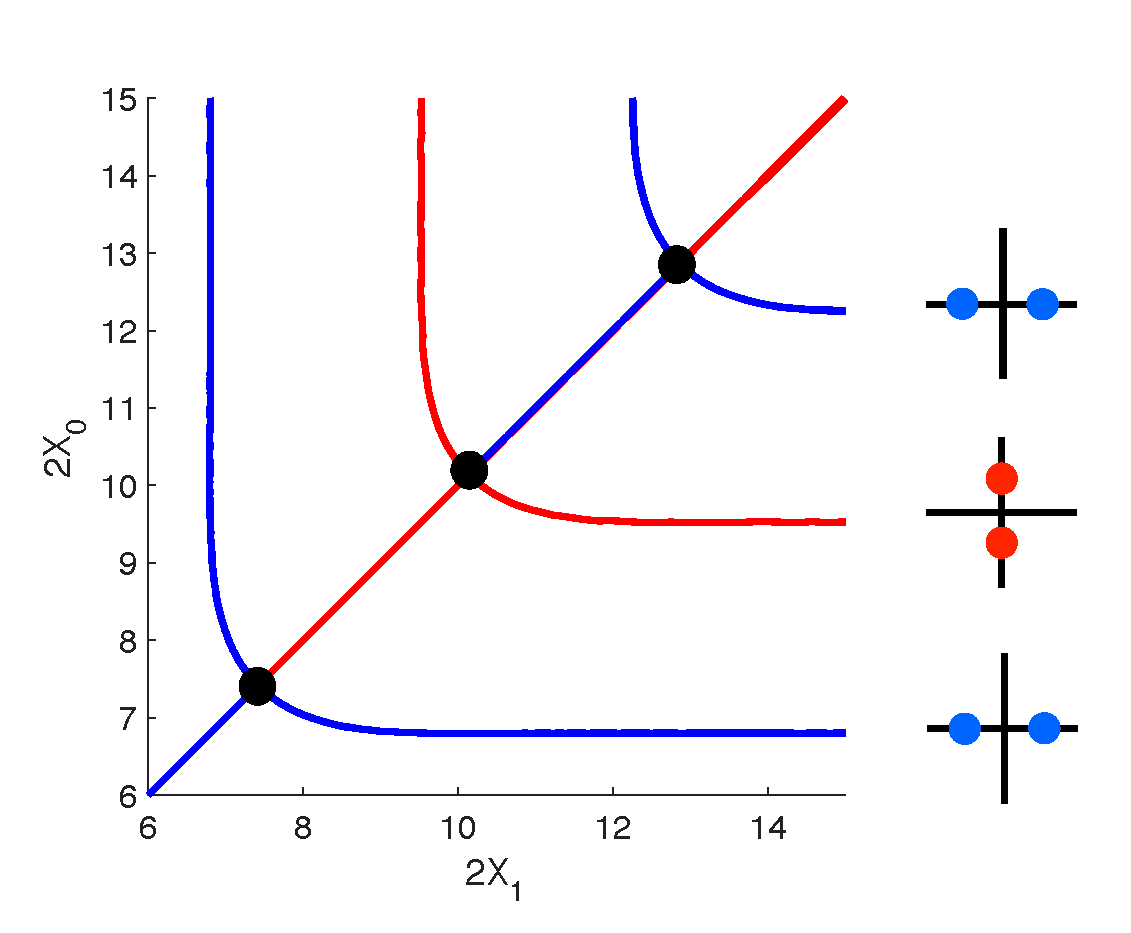
\includegraphics[width=10cm]{images/2periodiceigpattern.eps}
\end{center}
\caption[Interaction eigenvalue pattern for periodic double pulses in KdV5]{Interaction eigenvalue pattern for periodic double pulses. Blue lines represent periodic double pulses with a pair of real interaction eigenvalues. Red lines represent periodic double pulses with a pair of purely imaginary interaction eigenvalues. Bifurcations take place in the interaction eigenvalues at the black dots.}
\label{fig:2periodiceigpattern}
\end{figure}

Finally, we look at what happens when we increase the period $X$. For a neutrally stable double pulse, we have a pair of interaction eigenvalues on the imaginary axis whose location is approximately constant for large $X$. On the other hand, the essential spectrum eigenvalues \cref{Kdv5peress} move towards the origin as $X$ is increased. It is straightforward to determine the Krein signatures of the eigenvalues numerically; the interaction eigenvalues have negative Krein signature and the essential spectrum eigenvalues have positive Krein signature. At some value of $X$, these eigenvalues will collide. When this happens, since the eigenvalues have opposite Krein signatures, the two eigenvalues will generically move off of the imaginary axis and create an instability \cite[Chapter 7.1]{Kapitula2013}. By Hamiltonian symmetry, we expect there to be a pair of eigenvalues which has nonzero real part and is symmetric across the imaginary axis.

To see what happens in this case, we increase the periodic length parameter $X$ using AUTO. This is shown in \cref{fig:kreinbubble1}.
\begin{figure}
\begin{center}
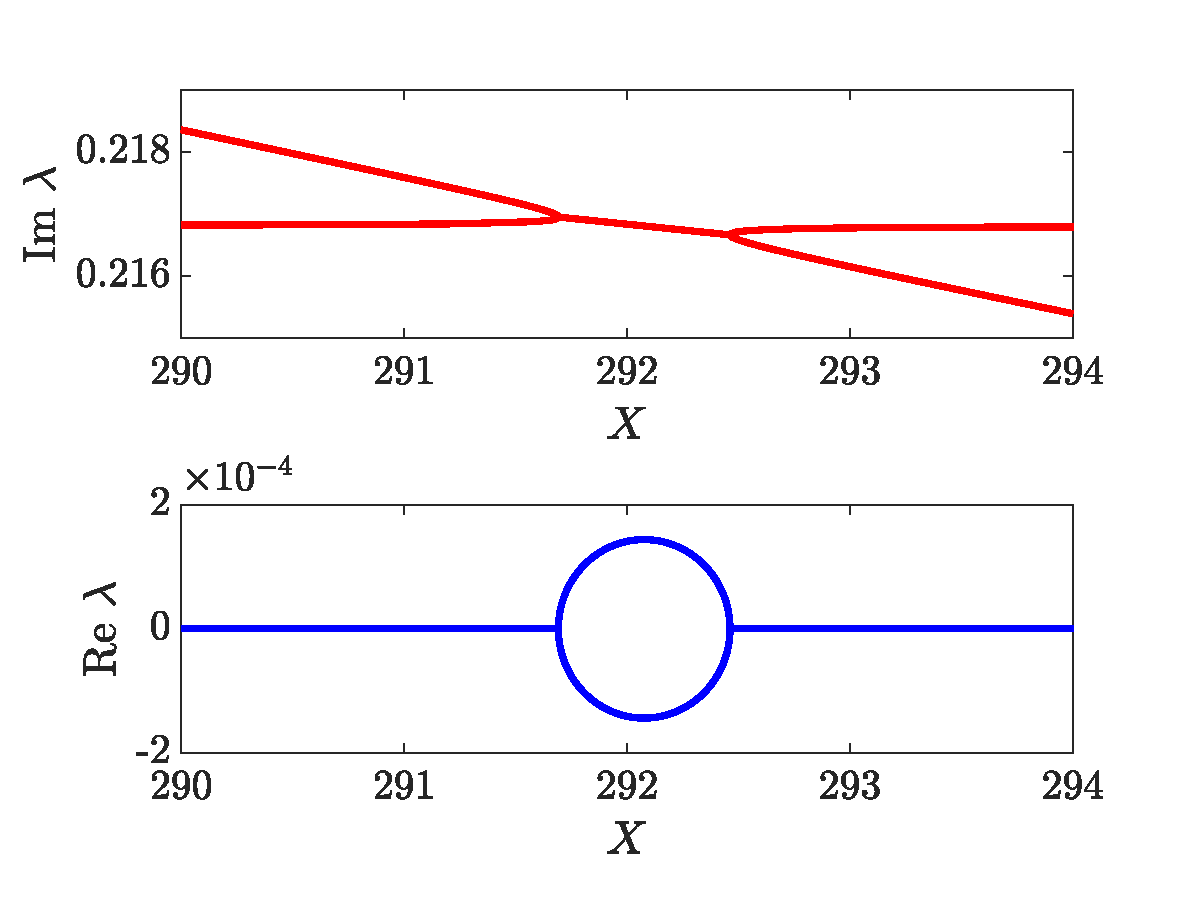
\includegraphics[width=10cm]{images/kreinbubble1}
\end{center}
\caption[Eigenvalue collisions for periodic double pulses in KdV5]{Collision of first essential spectrum eigenvalue with purely imaginary interaction eigenvalue as $X$ is increased. Imaginary part of eigenvalues on top, real part of eigenvalues on bottom. Parameter continuation with AUTO in periodic domain length $X$, $c = 20$.}
\label{fig:kreinbubble1}
\end{figure}
As $X$ is increased, the two eigenvalues undergo a Krein collision and move off of the imaginary axis. As $X$ is further increased, the eigenvalues come back together on the imaginary axis in a reverse Krein collision. Increasing $X$ further, the essential spectrum eigenvalue continues to move on the imaginary axis towards the origin, and the interaction eigenvalue is unchanged. We will call this instability bubble a Krein bubble. \cref{fig:kreinbubble1zoom} shows the eigenvalues of the Krein bubble in the complex plane. To leading order, the bubble is a circle.
\begin{figure}
\begin{center}
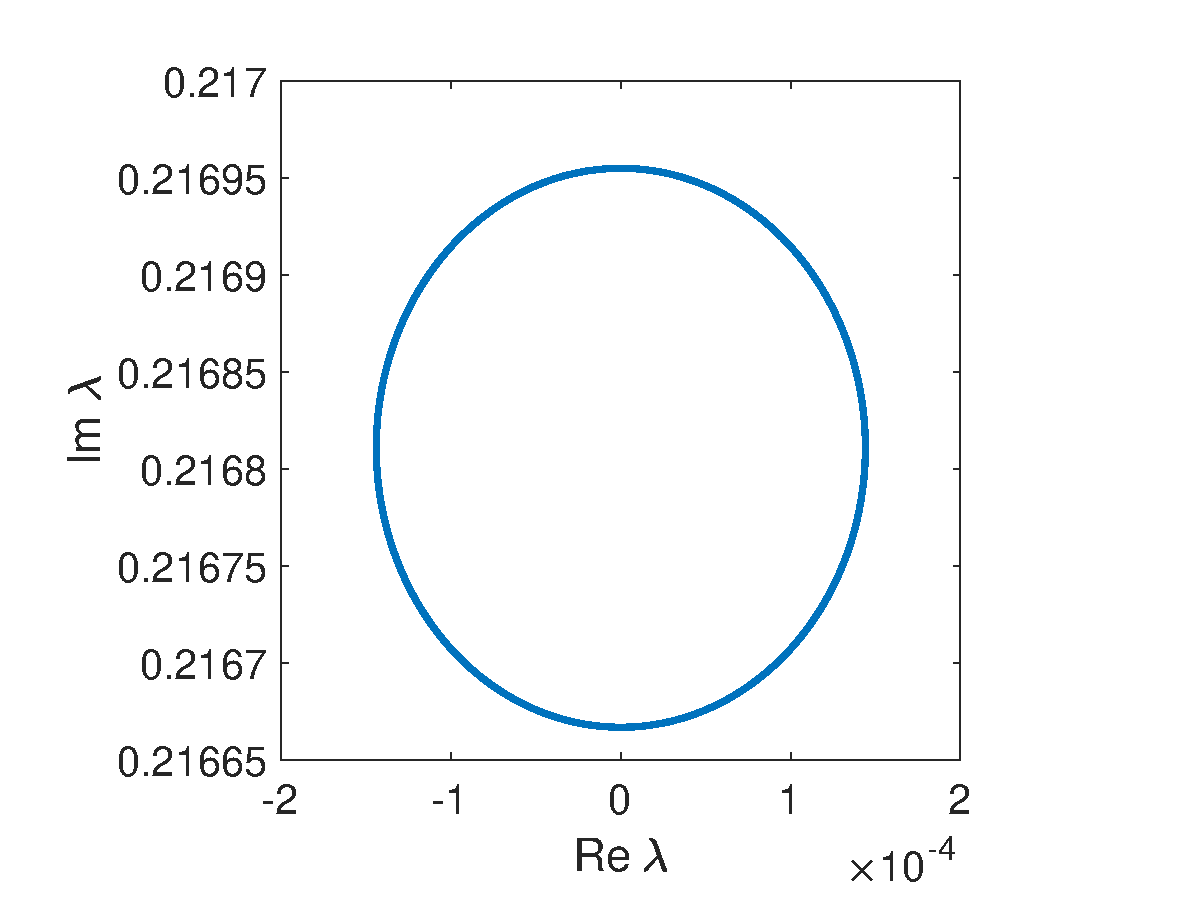
\includegraphics[width=8cm]{images/kreinbubble1zoom}
\end{center}
\caption[First Krein bubble for KdV5]{Plot of imaginary vs real part of eigenvalues inside Krein bubble occurring upon collision of first essential spectrum eigenvalue with interaction eigenvalue. $c = 20$.}
\label{fig:kreinbubble1zoom}
\end{figure}
For $c = 20$, the maximum real part of the eigenvalues in the Krein bubble is order order $10^{-4}$, which is very small compared to the interaction eigenvalue, which is approximately $0.22i$. We can continue the parameter continuation with AUTO, and we find a Krein bubble with every subsequent collision of an essential spectrum eigenvalue with the interaction eigenvalue. \cref{fig:kreinbubbleradius} plots the log of the Krein bubble radius versus the log of $X$ for the first 10 Krein bubbles.
\begin{figure}
\begin{center}
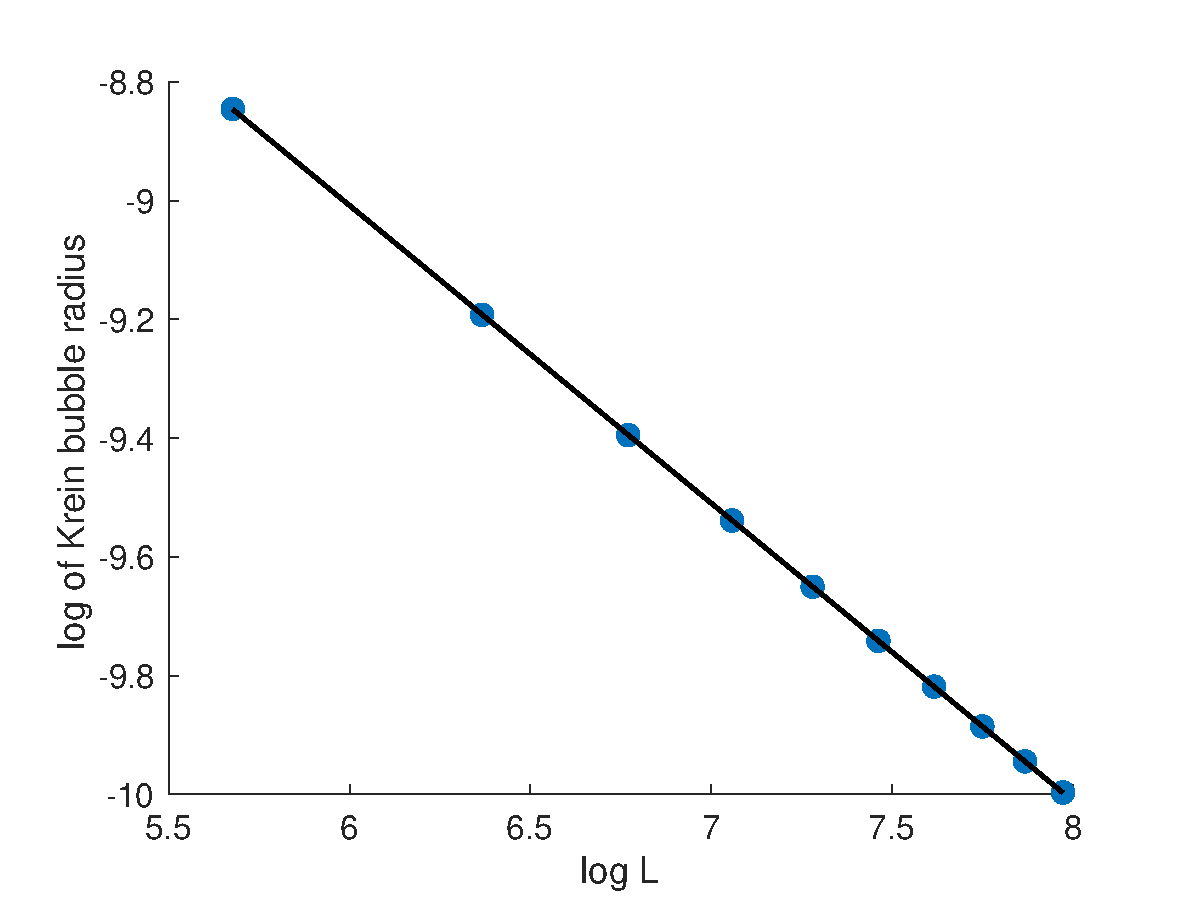
\includegraphics[width=8cm]{images/kreinbubbleradius}
\end{center}
\caption[Krein bubble radius for KdV5]{Plot of log of Krein bubble radius vs. log $X$ for the first 10 Krein bubbles together with least squares linear regression line. $c = 20$.}
\label{fig:kreinbubbleradius}
\end{figure}
The slope of the least squares linear regression line is $-0.5$ (with a relative error of less than $0.005$), which suggests that the radius of the Krein bubble scales as $X^{-1/2}$

\appendix
\section{Proofs of primary pulse results}
\section{Proofs of existence results}

Using \cref{nondegencond}, we decompose the tangent spaces of the stable and unstable manifolds at $Q(0; c_0)$. Since the two tangent spaces have a one-dimensional intersection spanned by $Q'(0; c_0)$, we can decompose them as 
\begin{equation}\label{TQ0decomp1}
\begin{aligned}
T_{Q(0; c_0)}W^u(0; c_0) &= \R Q'(0; c_0) \oplus Y^-(c_0) \\
T_{Q(0; c_0)}W^s(0; c_0) &= \R Q'(0; c_0) \oplus Y^+(c_0)
\end{aligned}
\end{equation}

For the variational equation, $DF(Q(x))$ is the $2m \times 2m$ matrix
\begin{equation}\label{defDF}
DF(Q(x)) = 
\begin{pmatrix}
0 & 1 & 0 & \dots & 0 & 0 \\
0 & 0 & 1 & \dots & 0 & 0 \\
& && \ddots \\
0 & 0 & 0 & \dots & 1 & 0 \\
0 & 0 & 0 & \dots & 0 & 1 \\
\partial_{u_1}f(Q(x)) - c & \partial_{u_2}f(Q(x)) & \partial_{u_3}f(Q(x)) & \dots & \partial_{u_{2m-1}}f(Q(x)) & \partial_{u_{2m}}f(Q(x))
\end{pmatrix}
\end{equation}

\begin{lemma}\label{eigadjoint}
Consider the linear ODE $V' = A(x)V$ and the corresponding adjoint equation $W' = -A(x)^* W$, where $A$ is an $n \times n$ matrix depending on $x$. Then the following are true.
\begin{enumerate}[(i)]
\item $\dfrac{d}{dx}\langle V(x), W(x) \rangle = 0$, thus the inner product is constant in $x$.
\item If $W(x)$ is bounded and $V(x) \rightarrow 0$ as $x \rightarrow \infty$ or $V(x) \rightarrow -\infty$, then $\langle V(x), W(x) \rangle = 0$ for all $x \in \R$. The same holds if we reverse the roles of $W$ and $V$.
\item If $\Phi(y, x)$ is the evolution operator for $V'(x) = A(x)V(x)$, then $\Phi(x, y)^*$ is the evolution operator for the adjoint equation $W'(y) = -A(y)^* W(y)$.
\end{enumerate}
\end{lemma}

\noi From \cref{eigadjoint}(ii), $\Psi(0) \perp \R Q'(0) \oplus Y^+ \oplus Y^-$, thus we can decompose $\R^{2m}$ as
\begin{equation}\label{R2mdecomp}
\R^{2m} = \R Q'(0) \oplus Y^+ \oplus Y^- \oplus \R \Psi(0).
\end{equation}

\section{Proofs of stability results}

\begin{equation}\label{PDEeigsystem}
V'(x) = A(U(x))V(x) + \lambda B V(x),
\end{equation}
where $A(U(x))$ is the $(2m+1)\times(2m+1)$ matrix
\begin{equation}\label{defAphi}
A(U(x)) = 
\begin{pmatrix}
0 & 1 & 0 & \dots & 0 & 0 & 0 \\
0 & 0 & 1 & \dots & 0 & 0 & 0\\
&  && \ddots \\
0 & 0 & 0 & \dots & 1 & 0 & 0 \\
0 & 0 & 0 & \dots & 0 & 1 & 0 \\
\partial_{u_1}f(U(x)) - c & \partial_{u_2}f(U(x)) & \partial_{u_3}f(U(x)) & \dots & \partial_{u_{2m-1}}f(U(x)) & \partial_{u_{2m}}f(U(x)) & 1 \\
0 & 0 & 0 & \dots & 0 & 0 & 0
\end{pmatrix}
\end{equation}


Using the nondegeneracy condition \eqref{nondegen2}, we can decompose the tangent spaces of the stable and unstable manifolds at $Q(0)$ as
\begin{align*}
T_{Q(0)}W^s(0) &= \R Q'(0) \oplus Y^+ \\
T_{Q(0)}W^u(0) &= \R Q'(0) \oplus Y^-
\end{align*}
Since $\dim \R Q'(0) \oplus Y^+ \oplus Y^- = 2m-1$, there we need two more directions to span $\R^{2m+1}$. 

Using Lemma \ref{nondegenlemma} and Lemma \ref{varadjsolutions}, we can decompose $\R^{2m+1}$ as  
\begin{equation}
\R^{2m+1} = \R \Psi(0) \oplus \R \Psi^c(0) \oplus \R Q'(0) \oplus Y^+ \oplus Y^-
\end{equation}
where $\R \Psi(0) \oplus \R \Psi^c(0) \perp \R Q'(0) \oplus Y^+ \oplus Y^-$.

\bibliographystyle{amsalpha}
\bibliography{kdv5.bib}

\end{document}
